\documentclass[a4paper,12pt]{scrbook}

\usepackage[utf8x]{inputenc}
\usepackage[T1]{fontenc}

\usepackage{amsmath}
\usepackage{amssymb}
\usepackage{amscd}
\usepackage{amsfonts}
\usepackage{amsthm}
\usepackage{graphicx}
%\usepackage{asymptote}
\usepackage{setspace}
\usepackage{version}
\usepackage[british]{babel}
\usepackage[pdfborder={0 0 0}]{hyperref}
%\usepackage{url}

\usepackage{mathtools}
\usepackage{pdfsync}

\usepackage{tikz}
\usetikzlibrary{snakes,arrows,shapes}

\usepackage{mathpartir}
\usepackage{listings}
\usepackage{stmaryrd}
\usepackage{synttree}

\usepackage{fancyhdr}

\usepackage[scaled]{beramono}

\usepackage[style=british]{csquotes}
\usepackage{pdfpages}
%\usepackage{subfigure}
\usepackage{subfig}

\usepackage{caption}

\captionsetup[figure]{name=Fig.}
%\captionsetup[table]{name=Tab.}

\theoremstyle{plain}
\newtheorem{theorem}[subsection]{Theorem}
\newtheorem{proposition}[subsection]{Proposition}
\newtheorem{lemma}[subsection]{Lemma}
\newtheorem{corollary}[subsection]{Corollary}
\newtheorem{conjecture}[subsection]{Conjecture}
\newtheorem{claim}{Claim}

\theoremstyle{definition}
\newtheorem{definition}[subsection]{Definition}
\newtheorem{note}[subsection]{Note}

\newcommand{\twofs}[2]{\genfrac{}{}{0pt}{1}{#1}{#2}}

\renewcommand{\leq}{\leqslant}
\renewcommand{\geq}{\geqslant}

\renewcommand{\labelenumi}{(\roman{enumi})}
%\onehalfspace
\parindent 5mm
\parskip   0mm

\newcommand{\sem}[1]{{\small{\textsf{#1}}}}
\newcommand{\tsem}[1]{\textsf{#1}}

\newcommand{\Mod}[1]{\;\text{mod}\,#1}
\newcommand{\icode}[1]{\texttt{#1}}
\newcommand{\sidecondition}[1]{\normalsize\textnormal{~ #1}}
\newcommand{\name}[1]{\textsf{#1}}
\newcommand{\proj}[2]{
  #2.\sem{#1}
}
\newcommand{\projd}[2]{
  \pi_{\textit{#1}} \left\llbracket #2 \right\rrbracket_{\Gamma, \Phi, \Sigma}
}
\newcommand{\denott}[2]{
  \left\llbracket \Gamma, \Phi \vdash #1 : #2 \right\rrbracket_{\Sigma}
}
\newcommand{\denottp}[2]{
  \left\llbracket \Gamma, \Phi \vdash #1 : #2 \right\rrbracket_{\Sigma'}
}
\newcommand{\denot}[1]{
  \left\llbracket #1 \right\rrbracket_{\Gamma, \Phi, \Sigma}
}

\newcommand{\sband}[0]{\overrightarrow\otimes}
\newcommand{\wedgedot}[0]{\,\ensuremath{\mathaccent\ldotp\wedge}\,}

\newcommand{\define}[0]{\triangleq}

\lstset{%
language=C,
basicstyle=\footnotesize\ttfamily,
keywordstyle=\footnotesize\bfseries\ttfamily,
% numbers=left,
numberstyle=\footnotesize,
% stepnumber=1,
% numbersep=5pt,
% backgroundcolor=\color{white},
showspaces=false,
showstringspaces=false,
showtabs=false,
frame=none,
tabsize=2,
captionpos=b,
mathescape=false
% breaklines=true,
% breakatwhitespace=false,
% escapeinside={\%*}{*)}
}

% Smaller url font
%% Define a new 'leo' style for the package that will use a smaller font.
\makeatletter
\def\url@smallstyle{%
  \@ifundefined{selectfont}{\def\UrlFont{\sf}}{\def\UrlFont{\footnotesize\ttfamily}}}
\makeatother
%\urlstyle{small}
\newcommand{\www}[1] {{\urlstyle{small}\url{#1}}}

\newcommand{\cc}[1]{{\text{\footnotesize\ttfamily{#1}}}}
\newcommand{\tcc}[1]{{\text{\ttfamily{#1}}}}
\newcommand{\ckw}[1]{{\text{\footnotesize\bfseries\ttfamily{#1}}}}

\newcommand{\comp}[0]{\cdot}
\newcommand{\lbracket}[0]{{\bfseries\texttt{[}}}
\newcommand{\rbracket}[0]{{\bfseries\texttt{]}}}

%opening
\title{Mathematizing the C Programming Language}
\author{Justus Matthiesen}

\begin{document}

%\maketitle

\thispagestyle{empty}
% \renewcommand{\headrulewidth}{0pt}
% \rhead[\bfseries Justus Matthiesen]{\bfseries\textsf{Justus Matthiesen}}
% \cfoot[]{}
\begin{flushright}
{\bfseries\textsf{Justus Matthiesen}\par}
\end{flushright}

\begin{center}
\null\vfill
 {\Huge {\bfseries\textsf{
Mathematizing the C Programming\\[1ex]
Language}
\par}}
{\vspace*{7cm}}
{\Large 
{Computer Science Tripos, Part II \par}
\vspace*{1ex}
{Gonville \& Caius College \par}
\vspace*{1ex}
{May 20, 2011 \par}
}
 \end{center}
 \null\vfill

\newpage
\thispagestyle{empty}
\mbox{}
\newpage
% \addtolength{\oddsidemargin}{-.8cm}
% \addtolength{\evensidemargin}{+.8cm}
\thispagestyle{empty}
\section*{Proforma}

\begin{tabular}{ll}
Name:		& {\bf Justus Matthiesen} \cr
College:	& {\bf Gonville \& Caius College} \cr
Project Title:	& {\bf Mathematizing the C Programming Language} \cr
Examination:	& {\bf Computer Science Tripos, Part II, June 2011} \cr
Word-count:	& {\bf 11,991 (as counted by TeXcount)} \cr
Project Originator:& {\bf Dr Peter Sewell} \cr
Project Supervisor:& {\bf Dr Peter Sewell}
\end{tabular}

\subsection*{Original aims of the project}
The goal of the project was to formalise a small fragment of the C programming
language, including at least integer arithmetic, and to produce a tool that
could be used as an oracle: Given a C program within the covered fragment, it
should output its meaning.

\subsection*{Work completed}
The formalisation of the language covers far more than the original proposal
suggested. It includes integer arithmetic, arrays, pointers, pointer arithmetic,
and more. The tool implementing the developed semantics produces and solves
logical statements describing the meaning of a given C program and,
additionally, it includes a type checking phase. Comparison of the tool output
with results produced by C compilers did not reveal any discrepancy for any of
the tested C programs.

\subsection*{Special difficulties}
None.

\subsection*{Declaration of Originality}
I, Justus Matthiesen of Gonville \& Caius College, being a candidate for Part II
of the Computer Science Tripos, hereby declare that this dissertation and the
work described in it are my own work, unaided except as may be specified below,
and that the dissertation does not contain material that has already been used
to any substantial extent for a comparable purpose.

\vspace{1\baselineskip}
    Signed

\vspace{1\baselineskip}
    Date: May 20, 2011

\tableofcontents

% Introduction + Preparation: ~3500 words.
\chapter{Introduction}\label{introduction}
We present a novel formalisation of a subset of C and describe the
implementation of a symbolic evaluator based on the newly developed semantics
capable of computing all behaviours of a (small) C program. The fundamental
motivation behind the project is the belief that the foundation of existing real
world computer systems should be provably solid; our semantics makes large parts
of the upcoming C1X standard precise, and our evaluator could be used as an
oracle for C compiler testing.

\section{A brief history of C}
The C programming language was created in the early 1970s by Dennis M. Ritchie
at the Bell Telephone Laboratories to fill the need of the new operating system
Unix for a system programming language \cite{developmentOfC}. The language
evolved into a general-purpose programming language over the next two decades
and its use spread so widely that a standardisation became necessary to avoid
the different dialects of C to diverge even further. Today, C is still an
evolving language: Since 2007 the ISO standards committee for the programming
language C has been preparing the newest revision of the C standard, called
C1X. It is expected to be finalised in the coming year.

% Over time the standard committee has laid out a number of general goals and
% guiding principles \cite{c1xCharter} that are meant to ensure that the spirit of
% C is maintained throughout the standardisation process. In the following, we
% will examine a few of these principles to help us understand the reasoning
% behind the design decisions that distinguish C from other languages.

\section{Underspecification and portability}
The first C implementation was written for the DEC PDP-11 architecture but it
has since been ported to a multitude of different architectures. To allow
programmers to target multiple architectures at the same time and to prevent C
from degenerating into a ``high-level assembly language'', the committee has
declared that C as defined by the standard must make it possible to write
programs whose behaviour is guaranteed to be independent of any particular
implementation and their underlying architecture (\textcquote{c1xCharter}{C can
  be portable}).

Unfortunately, portability is in conflict with C's original purpose as a systems
programming language: If the standard required, for example, consistent
behaviour in the case of integer overflows across different implementations, we
could no longer expect a compiler to be able to map a single C integer operation
to a single machine instruction. The compiler would have to account for the
difference between C standard and the specifics of the target
architecture. However, constant factors matter to the systems programmer and
hence hidden costs involved in the translation from C to machine code should be
kept at a bare minimum. The standard's solution to the conflict is to
underspecify behaviour when different architectures are likely to be
incompatible (\textcquote{c1xCharter}{make it fast, even if it is not guaranteed
  to be portable}).

To get a taste for the sometimes subtle consequences of underspecification,
consider the following program.
\lstinputlisting{examples/conversion.c}
%\caption{Implementation-defined behaviour due to integer type
%conversions.}\label{integerConversion}
If we tried to determine the outcome of the program without any knowledge of
the standard, we would expect the comparison always to be true. Indeed, if we
compile the program with any common C compiler on an x86-64 machine, the result
will be true. If we try the same program on a 32-bit x86 machine, however, the
program will return false. The discrepancy in behaviour is a consequence of
implicit type conversion, which we will discuss in detail at a later point.

\section{Aim of the project}
The previous discussion of underspecification should give an indication that
even very simple C programs have non-trivial semantics. Throughout the following
chapters we will examine a number of such programs that demonstrate how the C
language diverges from the programmer's intuition. Even those who have intricate
knowledge of the C standard often struggle with the subtleties of C, as
witnessed by the committee's internal mailing\footnote{ c.f. C -- Document
  register, \url{http://www.open-std.org/JTC1/SC22/WG14/www/documents} }
discussing what the correct interpretation of the standard should be, and by the
number of requests for clarification on the more ambiguous details of the
standard made in the form of defect reports\footnote{ c.f. WG14 Defect Report
  Summary for ISO/IEC 9899:1999,
  \url{http://www.open-std.org/jtc1/sc22/wg14/www/docs/summary.htm} }.

Like most standards, the C standard is written in natural language which,
despite the committee's great efforts to produce a precise description, is part
of the problem: A specification in natural language will unavoidably leave room
for vagueness and ambiguity. In contrast, a formal description of the language,
where we take ``formal'' to mean \textquote{admits logical reasoning}
\cite[p. 2]{norrishPhd}, would resolve the issue of
ambiguity. Underspecification, in particular, makes the behaviour of many
programs very difficult to predict without a formal model. Furthermore, a formal
understanding of C is especially desirable since the language is very widespread
in safety-critical applications.

The aim of this project is therefore to produce a formal description for part of
the C programming language. Unfortunately, to find such a description, we will,
like any other implementer, have to interpret the C standard first. If we are
not careful, misinterpretation of the standard will introduce inaccuracies into
the formalisation. As there is no way of proving that our derived semantics
captures the intent of the standard, it is also important that the semantics is
``recognisably'' a description of C. Hence, we consider it necessary to
formulate the semantics in a style that allows us to follow the definitions of
the standard as closely as possible.

Although it resolves ambiguity, a formal semantics alone cannot help us to
tackle the inherent complexity of C, since, even for fairly small programs, it
would be infeasible to determine their meaning by manual interpretation
according to the rules of the semantics. Instead, if we design the semantics to
be executable, we can write a program, namely a symbolic evaluator, based on the
pen-and-paper semantics that computes the meaning of a given C program. Since C
programs often exhibit non-deterministic behaviour, we could either design an
executable semantics that, when run, outputs just \textit{one} behaviour or a
semantics that considers \textit{all} behaviours at once. The potential
applications for a tool of the latter kind are plentiful: It could be used to
check whether a program contains undefined behaviour, it could be used as an
oracle in automatic compiler testing, or it could be used to empirically explore
how a change to the standard would affect the overall language.

\chapter{Preparation}
In this chapter, we discuss the scope of the project, explore what a formal
semantics for C must achieve, analyse the risks of particular implementation
strategies and examine the choice of development methodology.

\section{Scope of the project}
Our project covers a sizable fragment of C: In terms of general concepts, we
type check C programs and disambiguate overloaded operators. We faithfully model
the non-deterministic evaluation order including sequence points and the
sequenced-before relation. We also take into account the limited width of
integer types and express type conversions and integer overflows
precisely. Moreover, our semantics handles pointer and array types including the
alignment of memory addresses. Sadly, including a formal treatment of floating
point types would have gone beyond what can be done within the scope of this
project. We also excluded union, structure, and enumeration types as they come
with a large number of special cases in the language specification. However, our
semantics is expressive enough that they could be supported in principle.

We have defined and implemented rules for most of the expression language,
including recursive function calls and pointer arithmetic. We have no support,
however, for the syntactically heavy compound literals, generic selections, and
compound initializers. We opted not to model any of the bitwise operators apart
from the two shift operators since their behaviour is mostly
implementation-defined. Out of the statement language, we have support for all
of the iteration statements and, although our semantics does not give meaning to
the goto statement, our treatment of the continue, break and return statements
demonstrates that we are capable of expressing non-structural control-flow.

\section{Semantic engineering}
As outlined in the previous chapter, it is important that the formal description
closely resembles that of the standard. The standard defines the meaning of C
programs in a largely structural style, i.e., the definition is structurally
recursive in the grammar. As an example, consider how the behaviour of the
logical-and operator is specified.

\begin{figure}[htb]
\centering
\fbox{
\includegraphics[scale=0.8, page=117, trim=2.5cm 15.2cm 2cm 3.5cm, clip]{n1539}
}
\caption{Definition of the logical-and operator \cite[p. 99]{c1x}}
\label{land}
\end{figure}
The behaviour of the logical-and operator is recursively defined in terms of the
values of its operands, where \textit{logical-AND-expression} and
\textit{inclusive-OR-expressions} are non-terminal symbols of the expression
grammar. Fortunately, the different grammatical symbols only encode
associativity and operator precedence but otherwise do not carry any operational
meaning. As a consequence, we can work on an abstracted syntax instead.

\subsection{Problematic language features}\label{problematic}
Although C is defined in a largely structural style, it has a number of
properties and features that require us to use an unconventional semantic
style. We examine the most important of these in the following starting with
underspecification. Underspecification comes in three distinct flavours:
Implementation-defined, unspecified and undefined behaviour.

\subsubsection{Implementation-defined behaviour}
The behaviour of an operation is implementation-defined if the standard allows a
range of options but requires each implementation to make a consistent and
documented choice. For instance, the standard leaves it open whether the type
\lstinline{char} is a signed or an unsigned integer type. As a consequence, the
result of the program \lstinputlisting{examples/char.c} depends on which choice
an implementation makes. Since our aim is a semantics that is in direct
correspondence to the standard, we need to be careful that dependence on
implementation-defined behaviour is made explicit. After all, our semantics
should describe C and not just a specific implementation of C.

% Consider the following example program.
% \lstinputlisting{examples/intmax_cmp.c}
% One might expect the comparison always to be true, regardless of the value of
% \lstinline{i}. However, the value of expression \lstinline{i + 1} is converted
% to type \lstinline{int} before the comparison is evaluated. The value of
% \lstinline{i + 1} is outside the range of the type \lstinline{int}, in which case
% the standard rules the result of to be
% implementation-defined. The GCC C compiler, for example, converts the value by
% reducing it modulo $\text{\lstinline{INT_MAX}} + 1$
% \cite{gccImplementation}. For this particular choice, the conversion produces
% the value $1$, making the comparison false.

\subsubsection{Unspecified behaviour}\label{unspecifiedBehaviour}
Behaviour is unspecified if the standard presents several options without
imposing any further requirements on which is chosen in any circumstance.
Unspecified behaviour may seem very similar to implementation-defined behaviour,
but the key difference is that the former need not be the same on every run of a
program. The following program is an example of unspecified behaviour.
\lstinputlisting{examples/fg.c} Evaluation order in C is largely unspecified
with the result that either function call in expression \lstinline{f() + g()}
might be evaluated first. Thus, \lstinline{main} returns either $1$ or $2$,
which is unspecified.

As we will see shortly, the unspecified evaluation order of subexpressions is
especially problematic for many semantic styles since it causes sequential
programs like the above to behave non-deterministically.

\subsubsection{Undefined behaviour}
When a program containing undefined behaviour is executed, absolutely any
outcome is permitted: The program is semantically meaningless. It is the
programmers responsibility to keep programs free of undefined behaviour.

In many cases, undefined behaviour allows compilers to perform optimisation that
otherwise would require expensive analyses to guarantee safety. Division-by-zero
is such an example. \lstinputlisting{examples/divbyzero.c} A compiler is
allowed to assume that a program is free of division-by-zero errors since, if
otherwise, behaviour is undefined making any interpretation valid. Consequently,
compilers can perform code motion optimisation (even on architectures where
division by zero causes an exception) without having to perform the data-flow
analysis that ensures that all divisors are non-zero.

When dealing with undefined behaviour in a reduction semantics, we are faced
with two fundamental options: We could either introduce a special configuration
\textbf{undef}, say, and reduce all programs that exhibit undefined behaviour to
\textbf{undef} or we represent undefined behaviour as a stuck configuration,
i.e. we ensure that no program with undefined behaviour can be (fully) reduced
to a value. We believe that a semantics that implements the former option and
gives an explicit set of rules for undefined behaviour rather than defining it
\textquote{by omission of any explicit [...] behaviour} \cite[chapter 4,
§2]{c1x} is of greater value as it could be used to find the source of undefined
behaviour.

\subsubsection{Non-structural constructs}
Even though most of the language can be defined structurally, C has a range of
features whose meaning is context-dependent making them fundamentally
non-structural. Examples are the \lstinline{break} and \lstinline{continue}
statements inside loops but most strikingly the \lstinline{goto}
statement. Newer languages, like C\#\footnote{c.f. C\# Reference,
  \url{http://msdn.microsoft.com/en-us/library/13940fs2.aspx}.}, only allow
\lstinline{goto} statements that jump to labels that are lexically in scope. In
contrast, C only requires the label to be within the same function, which, for
instance, allows programs to execute both branches of the same
\lstinline{if}-statement.
\lstinputlisting{examples/goto.c}

\subsubsection{Memory model}\label{memoryModel}
The standard committee has decided to support multi-threaded program execution
in the next C standard. It will be based on the C++ memory model. Although we
will not include the memory model in our formal description, it is beneficial to
pick a semantic representation that allows it to be added in later without any
major modification of the semantics. The reason is that even sequential
C programs, as we have seen previously, can have non-deterministic behaviour. If
we view non-determinism as the general case rather than treating it as a special
case, we can hope to find a more uniform and concise specification of C.

\subsection{Choice of semantic style}
We now return to the question of semantic style. We summarise our reasons to
reject conventional semantic styles and give a contrasting, high-level overview
of our own semantics. For a full discussion we refer the reader to Appendix
\ref{semanticStyles}.

\subsubsection{Big-step semantics}
Since, in general, evaluation order is unspecified the order of evaluation of
subexpression $e_1$, $e_2$ and $e_3$ in
\begin{equation*}
\left( e_1 ~\cc{+}~ e_2 \right) ~\cc{+}~ e_3
\end{equation*}
can be any permutation of the three subexpressions. If $e_1$, $e_2$, $e_3$ are
side-effecting, then the order of evaluation can affect the result of the entire
expression. Hence, our semantics must be able to produce all of the (at least)
six evaluations of the above expression.

Big-step semantics forces us to make a choice of whether to fully evaluate the
left-hand or the right-hand operand of a binary operator first. The rules
\begin{equation*}
\inferrule* [Left=\textsc{[add-l]}, Right=\sidecondition{if $k = m + n$}] {
 \left< e_1, \sigma \right> \Downarrow \left< m, \sigma' \right>
 \\ \left< e_2, \sigma' \right> \Downarrow \left< n, \sigma'' \right>
} {
 \left< e_1 ~\cc{+}~ e_2, \sigma \right> \Downarrow \left< k, \sigma'' \right>
}
\end{equation*}
and
\begin{equation*}
\inferrule* [Left=\textsc{[add-r]}, Right=\sidecondition{if $k = m + n$ .}] {
 \left< e_1, \sigma' \right> \Downarrow \left< m, \sigma'' \right>
 \\ \left< e_2, \sigma \right> \Downarrow \left< n, \sigma' \right>
} {
 \left< e_1 ~\cc{+}~ e_2, \sigma \right> \Downarrow \left< k, \sigma'' \right>
}
\end{equation*}
express the two choices.

As a result, we cannot obtain the order $e_1$, $e_3$, $e_2$. If we reduce
expression $e_1$ first, then we must evaluate $e_2$ before we can evaluate
$e_3$:
\begin{equation*}
\inferrule* [Left=\textsc{[add-l]}] {
 \inferrule* [Left=\textsc{[add-l]}] {
   \left< e_1, \sigma \right> \Downarrow \left< m, \sigma_1
   \right>
   \\ \left< e_2, \sigma_1 \right> \Downarrow \left< m + n, \sigma_2
   \right>
 } {
   \left< e_1 ~\cc{+}~ e_2, \sigma \right> \Downarrow \left< m + n, \sigma_2
   \right>
 }
 \\ \left< e_3, \sigma_2 \right> \Downarrow \left< k, \sigma_3 \right>
} {
 \left< \left( e_1 ~\cc{+}~ e_2 \right) ~\cc{+}~ e_3, \sigma \right>
 \Downarrow \left< m + n + k, \sigma_3 \right>
} \quad.
\end{equation*}
It should be clear that this limitation makes big-step semantics a very poor
choice.

\subsubsection{Small-step semantics}
Whereas big-step semantics do not permit fine-grained control over the flow of
evaluation, small-step semantics give us the notion of a single computational
step. Although it resolves the issue of non-deterministic evaluation order in a
straightforward manner, the same cannot be said about non-structural language
features.

\subsubsection{Continuation semantics}
Continuation semantics, however, provide a neat framework for defining rules
that depend on their context. We have rules that produce evaluation contexts,
e.g.
\begin{equation*}
\inferrule* [Left=\textsc{[add-l]}, Right={,}] {} {
\left< e_1 ~\cc{+}~ e_2 \comp \kappa, \sigma \right> \rightarrow
  \left< e_1 \comp \left[ \_ ~\cc{+}~ e_2 \right] \comp \kappa, \sigma \right>
}
\end{equation*}
and also rules that destroy the context again:
\begin{equation*}
\inferrule* [Left=\textsc{[add-l-v]},
             Right=\sidecondition{if $v = v_1 + v_2$ .}] {} {
  \left< v_1 \comp \left[\_ ~\cc{+}~ v_2\right] \comp \kappa, \sigma \right>
    \rightarrow \left< v \comp \kappa, \sigma \right>
}
\end{equation*}

Again, we have to ensure that all possible evaluation orders of expression
$\left( e_1 ~\cc{+}~ e_2 \right) ~\cc{+}~ e_3$ are considered. Unfortunately,
the linear way in which we construct continuations prohibits certain evaluation
orders. We cannot, for example, evaluate $e_1$ first followed by $e_3$ since
after the first transition
\begin{equation*}
\left< \left( e_1 ~\cc{+}~ e_2 \right) ~\cc{+}~ e_3 \comp \textbf{stop},
       \sigma \right>
\rightarrow
\left< e_1 ~\cc{+}~ e_2 \comp \left[ \_ ~\cc{+}~ e_3 \right] \comp \textbf{stop},
       \sigma \right>,
\end{equation*}
expression $e_3$ is hidden inside the continuation and we cannot access it again
until $e_1 ~\cc{+}~ e_2$ has been reduced to a value.

\subsubsection{Trace semantics}\label{traceSemantics}
Unfortunately, there is no obvious solution to the above problem that does not
violate executability other than choosing a fundamentally different semantic
style.

In order to overcome the limitations of each of the choices above, we could use
a combination of several reduction relations, one for each semantic style, and
apply each to the expressions and statements they handle best. Whilst, as
Norrish \cite{norrishPhd} demonstrates, it is possible to express the whole of C
by using a range of different techniques, we would prefer a more uniform
description. Moreover, we still have to tackle two outstanding issues:
implementation-defined behaviour and support for a memory model.

Implementation-defined behaviour still stands in the way of executability. As an
illustration, consider the \lstinline{sizeof} operator. It tells us the size of
a given type in bytes\footnote{Even the number of bits in a byte is
  implementation-defined. According to the standard, it can be any number but
  must be at least eight.} but the standard only enforces a minimum
size. However, if we are to evaluate the expression \lstinline{sizeof(int)},
then the semantic styles we have discussed so far require us to either provide a
concrete number or sacrifice executability. Both are in direct conflict with our
initial goals.

It should be clear at this point that we will only be able to retain
executability if underspecification is mirrored in the language that we use to
describe the meaning of programs, e.g. \lstinline{sizeof(int)} must not be
reduced to a concrete number. Instead, it should be a symbolic value subject to
logical constraints encoding the requirements of the standard. Norrish's work is
a good demonstration. Since \name{Cholera} is implemented in the logic of the
HOL proof assistant, Norrish \cite[p. 30]{norrishPhd} can, for example, express
the fact that the number of bits in a byte is implementation-defined by simply
asserting
\begin{equation*}
\vdash \cc{CHAR\_BIT} \geq 8 ~.
\end{equation*}
Describing the meaning of programs within a logical framework gives us the
advantage that we can express underspecification naturally and still reason
about programs with implementation-defined behaviour.

%\textquote{[define] the set of values a read in a program is allowed to return,
%thereby defining the basic semantics of shared variables}
%\cite[p. 1]{memoryModels}.

Even though multi-threading will not be part of our semantics, we want our model
to be expressive enough to support it at least in principle. Multi-threaded
execution gives rise to weak ordering of accesses to shared memory. The memory
model specifies which orderings of memory actions are valid and which result in
undefined behaviour.
% It can be described as a binary relation on memory actions.
In concrete terms, we want to be able to apply our semantics for single-threaded
programs to several threads in isolation and specify the order of memory actions
at a later point.
%Consequently, our semantics must not make any assumptions when several distinct
%orderings of memory actions are valid with respect to the standard.
The implications for our semantics are twofold.

Firstly, when reading a shared memory object, we cannot provide a concrete value
since another thread might have altered the memory location since the last
write. As with implementation-defined behaviour, the issue can be resolved by
describing the meaning of programs within a logical framework: We associate a
symbolic variable with the result of the memory read giving us the option of
assigning a concrete value to it at a later stage with the knowledge of the
specific memory model in use.

Secondly, we have to expose shared memory accesses and the order in which they
occur to the memory model. Since even sequential C programs can have
non-deterministic behaviour, we can simplify our description of non-determinism
due to unspecified evaluation order by abandoning the notion of a global memory
completely and treating accesses to local memory in the same way as accesses to
shared memory. The key observation is that different choices in evaluation order
can only have an observable effect in the presence of side-effects: If both
operands of an addition are free of side-effects, then it does not matter which
operand is evaluated first. Hence, we could imagine an alternative semantics
that does not model the choice in evaluation order by a corresponding choice in
the next transition step (i.e. by defining a non-functional reduction relation)
but instead expresses it as an ordering relation on side-effects.  Unlike
before, the expression $e_1 ~\cc{+}~ e_2$ will no longer give rise to two
distinct evaluations. The unrestricted choice in evaluation order will instead
be expressed by a lack of ordering between the side-effects of the expression.

We illustrate the general idea using the following
program. \lstinputlisting[frame=none]{examples/traces/eqeq.c} In Figure
\ref{sbExample}, we present the ordering relation, or rather its transitive
reduction, on the program's actions as produced by our actual semantics. Actions
include all side-effects but also other events, e.g. $\sem{Id}_8(v_{48})$, for
reasons that we will explore in Section \ref{dynamicSemantics}.

Function \lstinline{main} declares two block scope identifiers \lstinline{x} and
\lstinline{y} of type \cc{int}. They become live at the start of the block and,
accordingly, action $\sem{Create}_2(\cc{int}, v_{48})$ and
$\sem{Create}_1(\cc{int}, v_{47})$ appear at the top of the graph. The arguments
$v_{48}$ and $v_{47}$ are symbolic names for the new memory locations of
\lstinline{x} and \lstinline{y}, respectively. Each action has an arbitrary but
unique label, here $2$ and $1$, so that they can always be distinguished. The
type information is necessary to inform the memory model of the size of the
object and to ensure that later reads and writes to the location adhere to the
relevant typing restrictions. Similarly, the following two memory writes
correspond to the initialisation of \lstinline{x} and \lstinline{y}. More
interestingly, in expression \lstinline{y = (x == x)}, the two loads from
\lstinline{x}, i.e $\sem{Load}_{11}(\cc{int}, v_{48}, v_{53})$ and
$\sem{Load}_{9}(\cc{int}, v_{48}, v_{51})$, can be executed in either order:
they are unrelated. Variables $v_{53}$ and $v_{51}$ are symbolic placeholders
for the values read from memory since we cannot provide concrete values until
after a total order on memory actions has been fixed. Action
$\sem{Store}_{12}(\cc{int}, v_{47}, v_{56})$ writes the result of the
comparison, $v_{56}$, to memory, whose value the semantics will further
constrain by a logical statement. Finally, $\sem{Kill}_4(v_{48})$ and
$\sem{Kill}_3(v_{47})$ announce the end of lifetime of identifiers \lstinline{x}
and \lstinline{y} to the memory model.

\begin{figure}[tb]
\centering
  \fbox{
    \begin{tikzpicture}[>=latex, scale=0.8]
      \tikzstyle{every node}=[font=\footnotesize]
      \input{examples/eqeq.c.main.tikz}
    \end{tikzpicture}
  }
\caption{Ordering relation on actions as produced by our semantics.}
\label{sbExample}
\end{figure}

A semantics of this kind can resolve all the complications that are inherent to
C reasonably well as we will see in Chapter \ref{chapter3}, where we present our
final semantics in full detail.


% Since evaluation order is mostly unspecified, we are faced with a
% combinatorial explosion in the number of evaluations we have to compute.

% In many programs and especially those with well-defined behaviour, most choice
% in evaluation order will not affect the observable behaviour. It seems
% therefore wasteful to treat all execution paths separately.
% \section{Tools and languages}
% \subsection{Ott and Isabelle}
% Originally, we planned to implement our semantics in the Isabelle/HOL proof
% assistant and use its code generation facilities to extract an executable
% version in form of an OCaml program afterwards.

% To ease the steep learning curve that comes with the use of proof assistants
% and to allow us, if necessary, to target a different proof assistant, we
% experimented with the Ott \cite{ott} tool. Ott has been designed to assist the
% formal definition of programming languages. It enables us to write syntax and
% semantics in a readable meta-language that has built-in support for notation
% commonly used in language definitions, e.g. BNF grammars, inductive relation
% defined using inference rules, and more. Given a definition in this
% meta-language, Ott can generate corresponding code for various proof
% assistants.  Using Ott for semantic definitions that follow one of the usual
% semantic styles works very well and, indeed, we were successful in expressing
% a partial version of our type system (c.f. Section \ref{staticSemantics}) in
% Ott. Sadly, our dynamic semantics makes extensive use of set operation which
% are not built into Ott.

% Initial experiments with code extraction revealed that an Isabelle/HOL
% formulation adequate for code generation would have to be far more intricate
% than anticipated. For example, it is not obvious how to generate meaningful code
% from non-functional reduction relations. The natural approach causes Isabelle's
% code generator \cite[p. 23]{codeGenerationManual} to produce a program that
% raises an exception when the result is not unique. Crucially, sets complicate
% code generation even
% further\footnote{See, for example, the following discussions on the Isabelle mailing list: \\
%   \url{https://lists.cam.ac.uk/pipermail/cl-isabelle-users/2011-March/msg00025.html},\\
%   \url{https://lists.cam.ac.uk/pipermail/cl-isabelle-users/2010-June/msg00103.html}.}.
% In order to avoid a shift in focus towards working with and around the
% particularities of a specific proof assistant, we decided to abandon the idea
% and, instead, opted for implementing the semantics in a functional programming
% language.

% \subsection{OCaml}
% It is well-known (c.f. \cite[p. 105]{zipperCFG} and \cite[p. 4]{modernCompiler})
% that programming languages of the ML-family are well-suited for writing programs
% that operate on abstract syntax trees (ASTs). We chose OCaml, in particular,
% because of its comparatively good tool support and availability of libraries.

% \subsubsection{Reuse of data structures and the expression problem}
% Compilers and other programs that transform syntax trees typically consist of
% several distinct phases which all operate on ASTs that only differ in small
% details. From a software engineering perspective, we would like to reuse those
% parts of the AST that are shared without sacrificing type safety. The problem is
% closely related to the expression problem proposed by Wadler: \blockquote{The
%   goal is to define a datatype by cases, where one can add new cases to the
%   datatype and new functions over the datatype, without recompiling existing
%   code, and while retaining static type safety} \cite{expressionProblem}. Our
% problem is a relaxed version of the expression problem since we allow
% recompilation.

% Traditionally, one represents an AST in OCaml using recursive variant
% types. Since variant types are closed, we cannot add more cases
% retrospectively. Furthermore, since constructor names must be unique, we cannot
% even expect functions defined for the one AST to work on a separate textual
% copy.

% It is possible to solve the expression problem with object-orientated techniques
% using inheritance and the visitor pattern. Unfortunately, the visitor pattern
% forces us to split code across many different classes and we are also no longer
% able to exploit pattern matching for tree transformations. Polymorphic variants
% are another option: They are open variant types that are flexible enough to
% solve the general expression problem but they, too, have disadvantages. Since
% they are open types, the compiler cannot detect, for example, misspelt
% constructor names.

% Since we are not willing to accept the implications for type safety and
% readability of the previous solutions, we opt for a partial solution due to
% Krishnaswami \cite{openVariant} that uses regular variant types.
% \lstinputlisting[language=ML]{examples/ocaml/rec.ml} The openly recursive type
% \lstinline[language=ML]{exp} only specifies the shape of the AST as all
% recursive arguments have been replaced by the type variable
% \lstinline[language=ML]{'e}. When tying the knot, we allow the AST to be
% augmented by an arbitrary annotation \lstinline[language=ML]{'a}. Thus, we can
% write functions that operate on ASTs with different annotations (c.f. function
% \lstinline[language=ML]{map_num}) but we still have to resort to textual copies
% if we want to add further cases.

\section{Development methodology}
Since the project proposal left a number of decisions open and since the
requirements imposed by C's unique set of features on the semantics still had to
be examined, we decided to adopt an iterative development process to allow an
explorative phase at the start of each cycle to refine the original development
targets. Formal development processes like Boehm's spiral model
\cite{spiralModel} have been mainly devised to guide large-scale software
development including interaction with a paying customer. The overhead involved
in fully adopting such a model would be overwhelming for a one-developer project
and a comparatively small time budget. Instead, we apply the principles of the
\textquote{\textit{risk-driven} approach} \cite[p. 61]{spiralModel} of the
spiral model in less formal procedure. After a first prototype that contained
common functionality, we implemented one feature at a time going through a
development cycle consisting of the following stages: initial experiments and
investigations to aid the requirement analysis, implementation, refactoring and
finally testing.

In addition, we make use of a range of tools to ensure development to go
smoothly. Most importantly, we use a version control system\footnote{Namely,
  \name{Mercurial} (\url{http://mercurial.selenic.com/}).} to facilitate
documentation and tracking of changes to the code base, to allow effortless
roll-backs and to enforce a strict separation of work-in-progress and production
code. To prevent disruption of development by data loss, automatic backups of
the local copy (containing unfinished and experimental work) and hosted
repository were performed\footnote{Using \name{rsync}
  (\url{http://rsync.samba.org/}) for incremental backups and the cron
  replacement \name{cronie} (\url{http://fedorahosted.org/cronie/}) for
  scheduling.} at regular intervals.

% Implementation: ~4500 words.
\chapter{Implementation}\label{chapter3}
Recall that the aim of our project is a tool that computes a logical statement
describing the meaning of a given source program. Implementing such a tool for C
is not an easy task: Parsing must not alter the semantics of the C program but
at the same time the result must be abstract enough to make the subsequent type
checking and semantic analysis feasible, the type checker has to cope with a
huge number of special cases, our dynamic semantics must be expressive enough to
model the subtle and often ambiguously defined behaviour of C operators, and
constraint solving has to be powerful enough to produce results but must be fast
enough to be practical. In this chapter we give an overview of the
implementation of this tool.
% Roughly, the work of the tool splits into the following phases: Lexing and
% parsing the input, transformation into an appropriate intermediate language,
% type-checking, semantic analysis and constraint solving. We describe each phase
% in chronological order and conclude with a look at the software design.

\section{Syntax}
Before we can analyse the semantics of a program, we must convert its plain
text description to an intermediate form that reveals the structure of the
program.

The standard describes what constitutes a syntactically correct program and how
to build the concrete syntax tree of a program in form of a BNF grammar.  As
usual much of the information encoded in the grammar, e.g. associativity and
precedence of operators, has the purpose to make parsing unambiguous. As we do
not want to complicate the subsequent semantic analysis unnecessarily, we
would like to work on an abstract syntax that ignores information that is only
relevant for parsing.

Our tool breaks the transformation into two distinct stages: The first parses C
programs to yield an intermediate representation that is still very close to the
original grammar. The second stage checks various syntactic constraints
on this intermediate representation and outputs the abstract syntax we use for
semantic analysis.


% Furthermore, some aspects of the grammar, like the declaration syntax,
% need to be transformed before we can determine their meaning.

% At the same time, we must not distance ourselves too far from it, since, as we
% observed in the previous chapter, the standard presents the semantics of C in a
% syntax-directed fashion.

\subsection{Parsing}\label{parsing}
Since the BNF is already a formal description of a language grammar, parsing was
not a priority and our project proposal planned to use the popular C front-end
\name{CIL} \cite{cil}. Despite that, we ended up writing our own parser.

\subsubsection{Why our own parser?}
Inspection of both the documentation and the source code revealed that
\name{CIL} was not suitable for our purposes: It not only parses input programs
but also performs a number of transformations that can alter the semantics of a
program. For example, \name{CIL} splits complex expressions into several smaller
pieces by use of temporary variables. Our example program demonstrating
unspecified behaviour (see Section \ref{unspecifiedBehaviour}), for instance, is
rewritten into one that is no longer non-deterministic. The new program
\lstinputlisting{examples/fg.cil.c} enforces left-to-right evaluation order and
thus eliminates the behaviour that arises from evaluating the function call to
\lstinline{g} first.

Another issue we observed resulted from a transformation that turns all implicit
type conversions into explicit type casts. The transformation requires the user
to provide \name{CIL} with the implementation-defined size of each integer type
and, depending on this information, \name{CIL} will produce different results.

These observations lead us to the conclusion that writing our own parser was
necessary.

\subsubsection{Parsing to an intermediate representation}
Apart from avoiding the deficiencies of existing front-ends, creating our own
parser gives us another advantage, as we will see below.

A grammatical C program is not necessarily a syntactically correct program. The
grammar allows, for example, functions to have storage class
\lstinline{register} but an additional syntactic constraint rules such programs
to be invalid. In our effort to stay close to the standard, we want our parser
to accept precisely those programs that are recognised by the BNF
grammar. Hence, in a first stage we parse to a low-level representation that is
still very close to the original grammar and then check syntactic constraints on
the intermediate representation, and translate it to an abstract syntax
appropriate for further analysis, in a second stage. Figure
\ref{grammarComparison} demonstrates that our parser indeed faithfully
reproduces the grammatical production of the standard.
\begin{figure}[hbt]
\centering
\subfloat{
\includegraphics[scale=0.86, page=480, trim=3cm 21cm 10cm 5cm, clip]{n1539}
}
\subfloat{
  \lstinputlisting[frame=none,language=ML,basicstyle=\footnotesize\ttfamily]
    {examples/ocaml/cast.mly}
}
\caption{Comparison of C grammar (left) and our parser (right).}
\label{grammarComparison}
\end{figure}

The strict separation of parsing and checking of other syntactic constraints
that mirrors the structure of the standard is only possible because we wrote our
own parser and did not choose a third-party front-end like \name{CIL}.

\subsection{From concrete to abstract syntax}\label{intermediateLanguage}
The second stage of the tool front-end generates abstract syntax from the
intermediate representation of the first stage. Many aspects of the
transformation are straightforward but, for example, the syntax of declarations
needs to be rewritten substantially before we can give a reasonable description
of their meaning.

In the following we will illustrate only some of the intricacies of transforming
the declaration syntax by use of a simple example.
\begin{figure}[bht]
\branchheight{1cm}
\childsidesep{0.3cm}
\synttree{10}[
\textit{declaration} [
  \textit{declaration-specifiers} [
    \textit{type-specifier} [.b
      \lstinline{int}
    ]
  ]
] [
  \textit{init-declarator-list} {\bfseries\texttt{;}} [
    \textit{init-declarator} [
      \textit{declarator} [
        \textit{direct-declarator} [
          \textit{direct-declarator} [
            {\bfseries\texttt{(}} \textit{declarator} {\bfseries\texttt{)}} [
              \textit{pointer} [.b
                {\bfseries\texttt{*}}
              ]
            ] [
              \textit{direct-declarator} [
                \textit{identifier} [.b
                  \texttt{a}
                ]
              ]
            ]
          ]
        ] [
          \lbracket \textit{assignment-expression} \rbracket [.x
            \texttt{3}
          ]
        ]
      ]
    ]
  ]
]
]
\caption{Derivation of \lstinline{int (* a)[3];}.}\label{derivationPointer}
\end{figure}
Figure \ref{derivationPointer} gives the full grammatical derivation of the
declaration \lstinline{int (* a)[3];}. The declaration introduces variable
\lstinline{a} and defines it to be a pointer to an integer array of size three.
From Figure \ref{derivationPointer} it should be apparent that the structure of
the derivations does not map very well to our intuitive understanding: A
declaration specifies the type of an identifier but the identifier is deeply
buried inside the grammatical structure of the type. And \lstinline{int} is
conceptually part of the array but it is grammatically completely
unrelated. Hence, our transformation needs to separate identifier and type
information and needs to bring the type information into a form that mirrors its
hierarchical structure. After transformation, our example will have the abstract
syntax tree given in Figure \ref{transformedPointer}.
\begin{figure}[tb]
\centering
\branchheight{1.2cm}
\synttree [
  \textit{type} [.b
    \texttt{POINTER}
  ] [
    \textit{type} [.b
      \texttt{ARRAY}
    ] [
      \textit{size} [.b
        \texttt{3}
        ]
    ] [
      \textit{type} [.b
        \texttt{INT}
      ]
    ]
  ]
]
\caption{Example \ref{derivationPointer} after transformation.}
\label{transformedPointer}
\end{figure}
Note how close the abstract syntax is to our prose description of the type.

Programmatically, we make extensive use of higher-order functions to rearrange
the parse tree. In particular, when faced with the grammar
production\footnote{To simplify matters, we will leave out the identifier
  \lstinline{a} from here on.} for array types, i.e.
\begin{equation*}
\textit{direct-declarator}
\rightarrow
\textit{direct-declarator} ~ \texttt{{\bfseries[}} ~
\textit{assignment-expression} ~ \texttt{{\bfseries]}} ,
\end{equation*}
we translate the \textit{direct-declarator} non-terminal to a function of type
\begin{equation*}
\left\llbracket \textit{direct-declarator} \right\rrbracket
: \texttt{AST.type} \rightarrow \texttt{AST.type} ~,
\end{equation*}
where \texttt{AST.type} is our abstract syntax representation of C types. Then
we can represent the entire production as the function composition of
$\left\llbracket \textit{direct-declarator} \right\rrbracket$ and a function
that, given a term of type \texttt{AST.type}, produces an array type of size
$\left\llbracket \textit{assignment-expression} \right\rrbracket$:
\begin{align*}
&\left\llbracket \textit{direct-declarator} ~ \texttt{{\bfseries[}} ~
\textit{assignment-expression} ~ \texttt{{\bfseries]}} \right\rrbracket : \texttt{AST.type} \rightarrow \texttt{AST.type} \define \\
&\quad \left\llbracket \textit{direct-declarator} \right\rrbracket \circ
\left(\lambda t : \texttt{AST.type} ~.~ \texttt{ARRAY} \left(\left\llbracket
    \textit{assignment-expression} \right\rrbracket,~ t\right)\right) .
\end{align*}
Finally, the rules for transforming pointer types,
\begin{equation*}
\left\llbracket \ckw{*} \right\rrbracket
 : \texttt{AST.type} \rightarrow \texttt{AST.type} \define
\lambda t : \texttt{AST.type} ~.~ \texttt{POINTER} \left( t \right) ~,
\end{equation*}
and the type specifier \lstinline{int},
\begin{equation*}
\left\llbracket \ckw{int} \right\rrbracket : \texttt{AST.type} \define \texttt{INT} ~,
\end{equation*}
are straightforward again. Putting it all together, we can now see how the AST
for the type declaration \lstinline{int (*)[3]} is generated\footnote{We cheat
  slightly in the first derivation step: To make the example presentable, we
  omitted describing the corresponding rule.}:
\begin{align*}
&\left\llbracket \ckw{int} ~ \cc{(} \ckw{*} \cc{)} \cc{[3]} \right\rrbracket \\
&= \left\llbracket \cc{(} \ckw{*} \cc{)} \cc{[3]} \right\rrbracket
\left\llbracket \ckw{int} \right\rrbracket \\
&= \left(\left\llbracket \cc{(} \ckw{*} \cc{)} \right\rrbracket \circ \left( \lambda t : \texttt{AST.type} ~.~ \texttt{ARRAY} \left(\texttt{3},~ t\right)
  \right)\right)\texttt{INT} \\
&= \left( \lambda t : \texttt{AST.type} ~.~ \texttt{POINTER}
  \left(\texttt{ARRAY} \left(\texttt{3},~ t\right)\right) \right) \texttt{INT}
\\
&= \texttt{POINTER}
  \left(\texttt{ARRAY} \left(\texttt{3},~ \texttt{INT}\right)\right) ~.
\end{align*}

To summarise, our implementation is a very concise description of the
non-trivial tree transformation due to the use of higher-order functions. We
leave it to the reader to imagine the stack-based implementation that would be
an appropriate choice in an imperative programming language like C without
first-class functions.

In this section we have looked at how to translate C programs to an intermediate
language suitable for semantic analysis. Most issues we faced originated from
the size and the unusual structure of C's grammar. Indeed, the syntax of C and
especially the declaration syntax has been a primary cause of criticism: As
Peter van der Linden puts it in his \textquote{Expert C Programming} book:
\textquote{the syntax of C declarations is a truly horrible mess that permeates
  the use of the entire language. It's no exaggeration to say that C is
  significantly and needlessly complicated because of the awkward manner of
  combining types.} \cite[p. 65]{expertC}.

\section{Static semantics}\label{staticSemantics}
The static semantics of C is not particularly complex in comparison to modern
typed languages like ML or Haskell: It lacks advanced features like implicit
polymorphism or type inference and the guarantees given by the type system are
very weak and not well understood. Because of this, our proposal did not
anticipate the need to implement the static semantics, but it was still
necessary: C operators are highly overloaded and hence, we need the type
information to disambiguate their use.

\subsection{Type checking}\label{typeChecking}
We will now examine the type system as used by our tool to annotate each node of
the AST with a type. We restrict the overview of our type system, which consists
of over 70 rules, to a handful of typeset and simplified rules that highlight
properties of the type system that are unique to C, rather then presenting the
actual OCaml implementation. The full type system requires a large number of
auxiliary functions and case distinctions to account for overloading, special
cases, and differently qualified types.

The type system of C can be described in the usual style: Our typing relation
has the general form $\Gamma, \Phi \vdash e : \tau$, where $e$ is an expression
and $\tau$ is a C type.  Moreover, the typing environment, $\Gamma$, is a
partial map from identifiers to types. Finally, $\Phi$ is the set of all
function names.

We begin with the base cases: An integer constant $n$ has type \cc{SIGNED INT}
provided it is within the range of values that can be represented by the type
\cc{SIGNED INT}.
\begin{equation*}
\inferrule* [Left=\textsc{[const]}] {
  \cc{INT\_MIN} \leq n \leq \cc{INT\_MAX}
} {
  \Gamma, \Phi \vdash n : \cc{SIGNED INT}
}
\end{equation*}
The standard only specifies a minimum range but the exact range is
implementation-defined. When $n$ is outside the minimum range, our
implementation enumerates all possible typings and remembers what assumptions,
e.g. $n \leq \cc{INT\_MAX}$, have been made for each.

Next, we look at identifiers. If an identifier $id$ has type $\tau$ according to
the type environment and is not a function name, then the type of the expression
is $\cc{lvalue}[\tau]$.
\begin{equation*}
\inferrule* [Left=\textsc{[id]}] {
  \Gamma(id) = \tau \\ id \not\in \Phi
} {
  \Gamma, \Phi \vdash id : \cc{lvalue} [ \tau ]
}
\end{equation*}
According to the standard an \textquote{\textit{lvalue} is an expression that
  can potentially designate an object}, where an object is a region of memory
that in most cases contains a value. If $id$ is a function name, then the result
is not an lvalue but will be a function type.
\begin{equation*}
\inferrule* [Left=\textsc{[id-fun]}] {
  \Gamma(id) = \tau \\ id \in \Phi
} {
  \Gamma, \Phi \vdash id : \tau
}
\end{equation*}
Unless an expression of function type $\tau$ is operand of the \lstinline{&} or
\lstinline{sizeof} operator, however, the expression will be coerced to type
pointer to $\tau$, i.e. $\cc{POINTER}(\tau)$. The fact that C does not have
first-class functions is reflected in the irregular behaviour of function types.
The rules do not allow function to be lvalues: The special identifier rule for
function names produces an expression type rather than lvalue type and, as we
will explore later, function pointers unlike other pointers cannot be turned
into lvalues.

The standard distinguishes between lvalue and expression types to account for
the asymmetric meaning of expressions in different contexts. An expression to
the left of an assignment operator is meant to represent the memory location
that is written to (hence the name \textit{l}value).
\begin{equation*}
\inferrule* [left=\textsc{[assign-arith]}] {
  \Gamma, \Phi \vdash e_1 : \cc{lvalue}[\tau_1] \\
  \Gamma, \Phi \vdash e_2 : \tau_2 \\
  \textit{is-modifiable}(\cc{lvalue}[\tau_1]) \\
  \textit{is-arithmetic}(\tau_1) \\
  \textit{is-arithmetic}(\tau_2) \\
} {
  \Gamma, \Phi \vdash e_1 \cc{ = } e_2 : \textit{unqualify}(\tau_1)
}
\end{equation*}
In most other contexts, we are interested in the value and not the memory
location of an object stored inside memory. We therefore must be able to convert
an lvalue type to a regular expression type when it occurs, for example, to the
right of an assignment operator:
\begin{equation*}
\inferrule* [Left=\textsc{[lvalue-conv]}, Right={.}] {
  \Gamma, \Phi \vdash e : \cc{lvalue} [ \tau ]
} {
  \Gamma, \Phi \vdash e : \textit{unqualify}(\tau)
}
\end{equation*}
To ensure that our rules coincide with an implementation, the choice of the next
rule in a type derivation must be strictly directed by the syntax of
expressions. Observe that the above rule breaks with the syntax-directed style
of the previous rules. It does not pose any restrictions on the form of
expressions $e$. In practice, we avoid the issue by inlining the rule wherever
necessary.

So far we have not mentioned the various auxiliary functions and predicates that
occur in the previous two rules. We restrict our presentation to a very brief
and informal description: Predicate \textit{is-arithmetic$(\cdot)$} is true for
all integer types\footnote{And floating types, but we do not model those.} and
\textit{is-modifiable$(\cdot)$} is true for lvalue types that are neither
\lstinline{const}-qualified nor array types. Finally, \textit{unqualify$(\tau)$}
is type $\tau$ but without any qualifiers.

The next topic of our overview is pointer types. Using the address operator
\lstinline{&}, we can turn any expression of lvalue type into a pointer, as
witnessed by the following typing rule:
\begin{equation*}
\inferrule* [Left=\textsc{[addr-lvalue]}, Right=\text{,}] {
  \Gamma, \Phi \vdash e : \cc{lvalue}[\tau] \\ \textit{is-object}(\tau)
} {
  \Gamma, \Phi \vdash \cc{\&} e : \cc{POINTER} (\tau)
}
\end{equation*}
where predicate \textit{is-object$(\cdot)$} is valid for all but function
types. The standard does, however, allow function pointers but since we cannot
have lvalues of function type, an extra rule is necessary, i.e.
\begin{equation*}
\inferrule* [Left=\textsc{[addr-fun]}, Right=.] {
  \Gamma, \Phi \vdash e : \tau \\ \textit{is-function}(\tau)
} {
  \Gamma, \Phi \vdash \cc{\&} e : \cc{POINTER} (\tau)
}
\end{equation*}
The indirection operator \lstinline{*} is the inverse of taking the address of
an object.
\begin{equation*}
\inferrule* [Left=\textsc{[indir-pointer]}] {
  \Gamma, \Phi \vdash e : \cc{POINTER}(\tau) \\ 
  \textit{is-object}(\tau)
} {
  \Gamma, \Phi \vdash \cc{*} e : \cc{lvalue}[\tau]
}
\end{equation*}
Again, function types need a special case that disallows the creation of
function objects.
\begin{equation*}
\inferrule* [Left=\textsc{[indir-fun]}] {
  \Gamma, \Phi \vdash e : \cc{POINTER}(\tau) \\ 
  \textit{is-function}(\tau)
} {
  \Gamma, \Phi \vdash \cc{*} e : \tau
}
\end{equation*}
We can now explain why speaking of ``function pointers'' is rather
misleading. Indirection on expressions of type pointer to function is an
idempotent operation: If the operand $e$ of the indirection operator has
function type $\tau$, the operand is, as we noted above, implicitly converted to
type $\cc{POINTER}(\tau)$. Hence, expression $e$ and, for example, $\cc{***}e$
both have type $\tau$. Thus, Norrish \cite[pp. 16f. and 23]{norrishPhd}
distinguishes between normal and function pointers at a type level reducing the
number of side-conditions and special cases. We decided against Norrish's
approach in order to stay close to the standard.

Finally, we examine typing rules for integer arithmetic. We start with the unary
\lstinline{+} operator.
\begin{equation*}
\inferrule* [Left=\textsc{[unary-plus]}] {
  \Gamma, \Phi \vdash e : \tau \\ \textit{is-arithmetic}(\tau)
} {
  \Gamma, \Phi \vdash \cc{+} e : \textit{promote}(\tau)
}
\end{equation*}
Operationally, the unary \lstinline{+} operator has no effect on the operand
other than \textit{promoting} its type. Integer promotion coerces an expression
to \lstinline{signed int}, if it has integer type whose range is a subset of the
\lstinline{signed int} type. The rationale is the following: An implementation
is meant to make the range of \lstinline{signed int} correspond to the register
size of the target architecture such that arithmetic operations on expressions
of type \lstinline{signed int} map directly to machine instructions. Hence,
integer promotions allow an implementation to use single machine instructions
for smaller integer types, too, without having to worry about overflows.

Similar type coercions are part of the binary arithmetic operations. The typing
rule for addition is for example:
\begin{equation*}
\inferrule* [left=\textsc{[add-arith]}, right=.] {
  \Gamma, \Phi \vdash e_1 : \tau_1 \\
  \Gamma, \Phi \vdash e_2 : \tau_2 \\
  \textit{is-arithmetic}(\tau_1) \\
  \textit{is-arithmetic}(\tau_2)
} {
  \Gamma, \Phi \vdash e_1 \cc{ + } e_2 : \textit{usual-arithmetic-conversion}(\tau_1, \tau_2)
}
\end{equation*}
The resulting type, \textit{usual-arithmetic-conversion$(\tau_1, \tau_2)$}, is
the \textit{common} type of \textit{promote$(\tau_1)$} and
\textit{promote$(\tau_2)$}. The common type of two arithmetic types is formed
according to a list of rules that have the purpose of selecting a type whose
range (in most cases) subsumes that of both types. Unfortunately, the rules for
determining a common type can have unexpected consequences when signed and
unsigned integer types are used within the same operation, as we have already
seen in Chapter \ref{introduction}.

\section{Dynamic semantics}\label{dynamicSemantics}
We have seen so far how our tool turns a given C program into a type-annotated
abstract syntax tree. The next phase in the tool pipeline consists of analysing
the dynamic semantics of a program: It transforms the type-annotated AST into a
logical description of the program's runtime behaviour.

The development of our dynamic semantics involved by far the greatest number of
design decisions. The result, unlike the previous stages, uses very little in
the way of standard techniques and style, required most creativity, and is
without a doubt the most novel part of this project.

\subsection{General form}\label{generalForm}
As we have outlined in Section \ref{traceSemantics}, in order to cope with
underspecification and non-deterministic behaviour, our dynamic semantics does
not compute concrete values. Instead, it accumulates logical constraints and
actions, including their ordering. More formally, we define a record\footnote{We
  borrow the notion of records from programming languages, using
  $\proj{\sem{\footnotesize{sequenced-before}}}{m}$, for example, for
  projection.} type
\begin{equation*}
   \begin{aligned}
    \sem{meaning} \define \big\{&\sem{actions} : \mathcal P (\sem{action});\\
    &\sem{function-actions} : \sem{action} \rightarrow \mathcal P (\sem{action}); \\
    &\sem{sequenced-before} : \mathcal P (\sem{action} \times \sem{action}); \\
    &\sem{constraints} : \sem{constraint} \big\} ,
  \end{aligned}
\end{equation*}
where the label \sem{constraints} is the crucial component. It is the logical
representation of the meaning of an expression $e$. All other components have
the purpose to make up for the lack of a global memory and to account for weakly
ordered memory actions (c.f. \ref{memoryModel}).

The component \sem{actions} is the set of all actions that occur in a particular
execution of $e$, where an action is either a memory read, a write, an
introduction of an object, an elimination of an object at the end of its
lifetime, or a function call\footnote{Modify corresponds to infix operations and
  id actions determine the identity of an lvalue.}:
\begin{align*}
  \sem{action} ::= ~&
  \sem{Store}_\textit{uid} (\tau, addr, \alpha) ~|~
  \sem{Load}_\textit{uid} (\tau, addr, id) ~|~
  \sem{Modify}_\textit{uid} (\tau, addr, \alpha, \alpha)  \\
&|~ \sem{Create}_\textit{uid}(\tau, id) ~|~
  \sem{Kill}_\textit{uid} (id)  \\
&|~ \sem{Id}_\textit{uid} (addr) ~|~
  \sem{Same}_\textit{uid} (addr, addr) \\
&|~ \sem{Call}_\textit{uid} .
\end{align*}
Each action is given a unique label $\textit{uid}$ to make them distinct.

We have already seen an example of the component \sem{sequenced-before} in
Fig. \ref{sbExample}: It is a non-reflexive, transitive order on the elements of
\sem{actions} (c.f. \ref{memoryModel}) encoding the evaluation order.  The last
component of the record, \sem{function-actions}, is an auxiliary ordering
constraint. It is a map from call actions to the set of actions that occur
in the execution of the corresponding function call.

With the definition of \sem{meaning} in place, we can describe the form of the
relation that defines the dynamic semantics: Given a typing $\Gamma, \Phi \vdash
e : \tau$ and a partial map, $\Sigma$, from program identifiers to symbolic
memory locations, the meaning of $e$ is a pair
\begin{equation*}
\denott {e} {\tau} : \sem{constant} \times \mathcal P (\sem{meaning}) .
\end{equation*}
The first component of the pair allows us to refer to the value produced by
expression $e$, where type \sem{constant} is the set of constants in our logical
framework (e.g. symbolic names, addresses or integers). Since a program often
has more than just one behaviour, the second component is a set of \sem{meaning}
records. We will sometimes speak of $m$-sets to refer to sets of type $\mathcal
P (\sem{meaning})$. Furthermore, see Table \ref{metaVars} for a list of
metavariables and their corresponding types.

\begin{table}[thb]
\centering
\fbox{
\begin{tabular}{ l l }
$a, a_1, \dots$           & \sem{action} \\
$\alpha, \alpha_1, \dots$ & \sem{constant} \\
$c, c_1, \dots$           & \sem{constraint} \\
$m, m_1, \dots$           & \sem{meaning} \\
$M, M_1, \dots$           & $\mathcal P (\sem{meaning})$ \\
$u, u_1, \dots$           & \textit{uid}
\end{tabular}
}
\caption{List of metavariables}\label{metaVars}
\end{table}

Above we have consciously avoided mentioning statements. Unlike expressions,
statements do not produce values but otherwise there is little conceptual
difference between the two. Hence, the semantics of statements can be seen as a
special case of the expression semantics:
\begin{equation*}
\denott {s} {\cc{void}} : \mathcal P (\sem{meaning}) .
\end{equation*}

% Before we can give rules for the various C operators, we need to introduce
% notational conventions: We list metavariables and their corresponding type in
% table \ref{metaVars}.

\subsection{Expression semantics}
In this section, we present our dynamic semantics for expressions using a
selection of rules that demonstrate how we resolve the issues related to
evaluation order, undefined behaviour, implementation-defined behaviour,
implicit type conversions, and the interaction with a memory model. We begin
with the base cases for integer constants and identifiers.

\subsubsection{Base cases}
An integer constant $n$ has, of course, no side-effects, no control-flow, and
its value is unconditionally just $n$\footnote{For notational convenience, we
  will often omit the parentheses around pairs in future.}:
\begin{equation*}
\inferrule* [Left=\textsc{[const]}, Right={,}] {} {
   \denott {n} {\tau} = \left(n, \sem{empty}\right)
}
\end{equation*}
where \sem{empty} is the singleton set
\begin{equation*}
  \begin{aligned}
    \sem{empty} \define \Big\{ \big\{
    &\sem{actions} = \left\{\right\} ; \\
    &\sem{compound-actions} = \left\{\right\} ; \\
    &\sem{function-actions} = \left\{\right\} ; \\
    &\sem{sequenced-before} = \left\{\right\} ;\\
    &\sem{constraints} = \sem{true}  \big\} \Big\} .
  \end{aligned}
\end{equation*}
For other rules, we need to be able to add further constraints and actions to
each element in a set $M$. Again, we borrow notation from programming languages:
$\left\{m \textit{ with } \sem{constraints} = c \right\}$ is record $m$ with
component \sem{constraints} replaced by $c$. Using this notation, adding a
constraint is simply
\begin{equation*}
m \wedge c \define
  \left\{m \textit{ with } \sem{constraints} =
    \proj{constraints}{m} \wedge c
  \right\} .
\end{equation*}
Similarly,
\begin{equation*}
m \wedgedot a \define
  \left\{m \textit{ with } \sem{actions} =
    \proj{actions}{m} \cup a
  \right\} .
\end{equation*}
We lift both operations to the set level in the obvious way, i.e.
\begin{equation*}
M \wedge c \define
  \left\{m \wedge c \vert m \in M \right\}
\end{equation*}
and
\begin{equation*}
M \wedgedot a \define
  \left\{m \wedgedot a \vert m \in M \right\} .
\end{equation*}
In order to reduce the number of parentheses necessary, we will assume that
operators $\otimes$ and $\sband$ (to be introduced later) are more tightly
binding than $\wedge$ and $\wedgedot$ and that $\wedge$ and $\wedgedot$
associate to the left.

Now, we can specify the second base case. An identifier $id$, that does not
designate a function, represents a memory object. In a non-lvalue context, it
denotes the contents of the object, i.e. it loads the value residing at
location $\Sigma(id)$ from memory:
\begin{equation*}
\inferrule* [Left=\textsc{[id]}, Right=\sidecondition{$\alpha$, \textit{u} fresh .}] {
  id \not\in \Phi
} {
   \denott {id} {\tau} =
     \alpha,
     \sem{empty} \wedgedot \sem{Load}_{\textit{u}}(\tau, \Sigma(id), \alpha)
}
\end{equation*}
The exact value for the fresh name $\alpha$ will be provided later by the memory
model in form of an additional constraint (e.g. $\alpha = \cc{3}$).

If, however, the identifier appears in an lvalue-context, it denotes the
memory location $\Sigma(id)$. We use a separate functions, $\denott{e}{\tau}$ and $\denott{e}{\tau}^{\textit{lvalue}}$, to represent the
semantic split between value- and lvalue-producing contexts. In particular,
\begin{equation*}
\inferrule* [Left=\textsc{[lvalue-id]}, Right={.}] {
  id \not\in \Phi
} {
   \denott {id} {\tau}^{\textit{lvalue}} =
     \Sigma(id), \sem{empty}
}
\end{equation*}

\subsubsection{Integer arithmetic}\label{arithmetic}
Next we turn to inductive rules. Since our semantics is recursive in the
structure of expressions, we often have to combine the meaning of two
subexpressions. For instance, expression $e_1 \cc{+} e_2$ has exactly the
actions of its subexpressions, it has at least the constraints of $e_1$ and
$e_2$, and evaluation order is unrestricted, i.e. the actions of $e_1$ are not
related to $e_2$ by the \sem{sequenced-before} relation\footnote{We will say
  \textit{unsequenced} from here on.}. The following definition expresses this
operation for records $m_1$ and $m_2$.
\begin{equation*}
  \begin{aligned}
    m_1 \otimes m_2 \define \big\{ 
    &\sem{actions} = \proj{actions} {m_1} \cup \proj{actions} {m_2} ; \\
    &\sem{compound-actions} =
      \proj{compound-actions} {m_1} \cup \proj{compound-actions} {m_2} ; \\
    &\sem{function-actions} =
      \proj{function-actions} {m_1} \cup \proj{function-actions} {m_2} ; \\
    &\sem{sequenced-before} = 
      \proj{sequenced-before} {m_1} \cup
      \proj{sequenced-before} {m_2} ; \\
    &\sem{constraints} =
      \proj{constraints} {m_1} \wedge \proj{constraints}{m_2} \big\}
  \end{aligned}
\end{equation*}
As before, we lift the operation to sets of such records:
\begin{equation*}
M_1 \otimes M_2 \define \left\{
  m_1 \otimes m_2 \vert \left( m_1, m_2\right) \in M_1 \times M_2
\right\} .
\end{equation*}

With these operators at our disposal, we can give the semantics for the (signed)
addition of two integers.
\begin{equation*}
\inferrule* [Left=\textsc{[add]}, Right=\sidecondition{$\alpha$ fresh}] {
  \textit{is-arithmetic}(\tau_1) \\
  \textit{is-arithmetic}(\tau_2) \\
  \textit{is-signed-arithmetic}(\tau) \\\\
  \denott {e_1} {\tau_1} = \left(\alpha_1, M_1\right) \\
  \denott {e_2} {\tau_2} = \left(\alpha_2, M_2\right)
} {
   \denott {e_1 \cc{ + } e_2} {\tau} =
    \alpha,
    \left( M_1 \otimes M_2 \right) \wedge
      \left(
        \alpha =
          \sem{conv}_\tau(\alpha_1) + \sem{conv}_\tau(\alpha_2)
        \wedge \neg\sem{range}_\tau (\alpha) \rightarrow \sem{undef}
      \right)
}
\end{equation*}
Since addition is overloaded (pointer arithmetic uses the same operator), we
have to check first that both operands really are integers. Before the values of
the two operands are added, the standard requires us to convert both operands to
their common type but as we only operate on well-typed programs we know that
$\tau$ is already the common type (c.f. Section \ref{typeChecking}) of $\tau_1$
and $\tau_2$. Here, we use the notation $\sem{conv}_{\tau}(\cdot)$ as a
shorthand for the type conversion. In the case $\tau=\cc{UNSIGNED INT}$, for
example, we would expand it to
\begin{equation*}
\sem{conv}_{\text{\scriptsize\ttfamily{UNSIGNED INT}}} \left( \alpha \right)
\define \alpha \Mod \cc{UINT\_MAX} .
\end{equation*}
Finally, if the result of the (usual mathematical) addition, is outside the
range of integers that can be represented by signed type $\tau$, then behaviour
is undefined according to the standard. Again, $\sem{range}_\tau(\cdot)$ is a
shorthand that in our actual implementation is replaced by a type-specific
condition, e.g. $\cc{INT\_MIN} \leq \alpha \wedge \alpha \leq
\cc{INT\_MAX}$. Term $\sem{undef}$ is a special nullary predicate that indicates
undefined behaviour.

The corresponding rule for signed integer addition only differs in the treatment
of overflows. Unsigned integer overflows do not exhibit undefined behaviour but
instead the resulting value, $\alpha$, is reduced modulo the largest integer
representable by $\tau$, e.g. \cc{UINT\_MAX}.

So far we have only looked at rules that do not impose any restrictions on
evaluation order. In contrast, the logical-and operator uses a strict
left-to-right evaluation strategy: In $e_1 \cc{\&\&} e_2$, the actions of $e_1$
are sequenced before those of $e_2$. Consequently, we can no longer use operator
$\otimes$ to combine the $m$-sets of the two subexpressions as it assumes
evaluation order to be unspecified. Hence, we define a non-commutative operator
that inserts a \sem{sequenced-before} dependency between each pair of actions
$\left(a_1, a_2\right)$ where $a_1$ occurs in $m_1$ and $a_2$ in $m_2$:
\begin{equation*}
  \begin{aligned}
    m_1 \sband m_2 \define \big\{
    &\sem{actions} = \proj{actions} {m_1} \cup \proj{actions} {m_2} ; \\
    &\sem{compound-actions} =
      \proj{compound-actions} {m_1} \cup \proj{compound-actions} {m_2} ; \\
    &\sem{function-actions} =
      \proj{function-actions} {m_1} \cup \proj{function-actions} {m_2} ; \\
    &\sem{sequenced-before} =
      \proj{actions}{m_1} \times \proj{actions} {m_2} \\ &\quad \cup
      \left(\proj{sequenced-before} {m_1} \cup
        \proj{sequenced-before} {m_2}\right) ; \\
    &\sem{constraints} =
      \proj{constraints} {m_1} \wedge \proj{constraints}{m_2}  \big\} .
  \end{aligned}
\end{equation*}
Lifting to $m$-sets, gives us
\begin{equation*}
M_1 \sband M_2 \define \left\{
  m_1 \sband m_2 \Big\vert \left( m_1, m_2\right) \in M_1 \times M_2
\right\} .
\end{equation*}
Recall from the definition in Fig. \ref{land} that C's logical-and operator also
has non-trivial control-flow: The second expression is only executed if the
first expression does not evaluate to $0$. Fortunately, our choice of semantic
style makes branching control-flow a non-issue: each element of an $m$-set
represents a (potentially) distinct execution path. The $m$-set associated with
$e_1 \cc{\&\&} e_2$ can therefore be described as the union of two $m$-sets,
where the first,
\begin{equation*}
M_1 \wedge \alpha_1 = 0 \wedge \alpha = 0,
\end{equation*}
corresponds to the case when only $e_1$ is evaluated and the second $m$-set,
\begin{equation*}
  M_1 \sband M_2 \wedge \alpha_1 \not= 0 \wedge \alpha = \left( \alpha_2 \not= 0
    \rightarrow 1 \vert 0\right),
\end{equation*}
represents the case when both subexpressions are evaluated:
\begin{equation*}
  \inferrule [\textsc{[land]}] {
    \denott {e_1} {\tau_1} = \left(\alpha_1, M_1\right) \\
    \denott {e_2} {\tau_2} = \left(\alpha_2, M_2\right) \\
    \sidecondition{$\alpha$ fresh}
%    \alpha ~ \text{fresh}
  } {
    \denott {e_1 \cc{ \&\& } e_2} {\tau} =
    \alpha,
    M_1 \wedge \alpha_1 = 0 \wedge \alpha = 0
    \cup M_1 \sband M_2 \wedge \alpha_1 \not= 0
      \wedge \alpha = \left( \alpha_2 \not= 0 \rightarrow 1 \vert 0\right)
  }
\end{equation*}
We use the notation\footnote{Following Gordon's lectures notes on
  \textquote{Specification and verification I}:
  \url{http://www.cl.cam.ac.uk/~mjcg/Teaching/SpecVer1/Notes/Notes.pdf}.}
$\left(p \rightarrow \alpha_1 \vert \alpha_2 \right)$ to say ``if $p$ holds then
$\alpha_1$ else $\alpha_2$''.

\subsubsection{Assignments}
Lvalue-contexts occur in the simple and compound assignment, pre- and postfix
increment, and the address operator but, here, we only present the rule for the
simple assignment operator (on arithmetic types). The expression to the left of
the assignment must evaluate to an lvalue. We therefore use $\denott{e_1}
{\tau_1}^{\textit{lvalue}}$ in the premise of the assignment rule instead of the
usual value-producing semantic function:
\begin{equation*}
  \inferrule* [Left=\textsc{[assign]}, Right=\sidecondition{$\alpha$,
    \textit{u} fresh}] {
    \textit{is-arithmetic}(\tau_1) \\
    \textit{is-arithmetic}(\tau_2) \\\\
    \denott {e_1} {\tau_1}^{\textit{lvalue}} = \left(\alpha_1, M_1\right) \\
    \denott {e_2} {\tau_2} = \left(\alpha_2, M_2\right) %\\
  } {
    \denott {e_1 \cc{ = } e_2} {\tau} =
    \alpha,
    \left(M_1 \otimes M_2\right) \sband \left(\sem{empty} \wedgedot
      \sem{Store}_{\textit{u}} \left(\tau, \alpha_1, \alpha\right)\right) \wedge \alpha =
      \sem{conv}_\tau (\alpha_2)
    }
\end{equation*}
Hence, $\alpha_1$ in the above rule denotes a symbolic memory location and can
be used as the address argument of the load action.

Also note that, according to the standard, the actions of the two subexpressions
are unsequenced with respect to each other, i.e.
\begin{equation*}
M_1 \otimes M_2 .
\end{equation*}
They are both, however, sequenced before the write to memory and therefore
\begin{equation*}
\left(M_1 \otimes M_2\right) \sband \left(\sem{empty} \wedgedot
  \sem{Store}_{\textit{u}} \left(\tau, \alpha_1, \alpha\right)\right) .
\end{equation*}

\subsubsection{Pointers and pointer arithmetic}\label{pointerArithmetic}
The ability to take the address of any object is essential to the character and
spirit of C. The lack of restrictions in taking addresses (e.g. returning the
address of a local variable is not a compile-time error) and pointer arithmetic
distinguishes C from many other programming languages and is a very common cause
of security-relevant software bugs.

The rules for the two main pointer operations, the address and indirection
operators, are closely related. The address operator determines the memory
location of the object denoted by its operand:
\begin{equation*}
  \inferrule* [Left=\textsc{[addr]}, Right={.}] {
    \denott {e} {\tau}^{\textit{lvalue}} = \alpha, M \\
    \neg \exists e' . e \equiv \cc{*} e'
  } {
    \denott {\cc{\&} e} {\tau} = \alpha, M
    }
\end{equation*}
The indirection operator can be seen as the inverse of the address operator. It
turns its operand which must be of pointer type into an lvalue:
\begin{equation*}
  \inferrule* [Left=\textsc{[indir-lvalue]}, Right={.}] {
    \denott {e} {\tau} = \alpha, M
  } {
    \denott {\cc{*} e} {\tau}^{\textit{lvalue}} = \alpha, M
      \wedge \left(\alpha = \sem{null} 
          \vee \neg\sem{align}_{\tau}(\alpha)\right) \rightarrow \sem{undef}
  }
\end{equation*}
In fact, the standard states that expression $\cc{\&*}e$ is equivalent to $e$
even if $e$ evaluates to a null pointer. Hence, the rule \textsc{[addr]}
excludes the case when $e$ is an indirection operator. The indirection rule also
expresses that behaviour is undefined if either the operand evaluates to a null
pointer or the pointer has the wrong alignment.

We conclude the section with a short discussion of pointer arithmetic.
\begin{equation*}
  \inferrule* [Left=\textsc{[add-ptr]},
               Right=\sidecondition{\textit{u} fresh.}] {
    \tau = \cc{POINTER}(\tau_1) \\
    \textit{is-integer}(\tau_2) \\\\
    \denott {e_1} {\tau}  = \alpha_1, M_1 \\
    \denott {e}  {\tau_2} = \alpha_2, M_2
  } {
    \denott {e_1 \cc{+} e_2} {\tau} =
      \alpha, M_1 \otimes M_2
        \wedge \alpha = \alpha_1 + \alpha_2 * \sem{sizeof}_{\tau_1}
        \wedgedot \sem{Same}_u(\alpha_1, \alpha)
  }
\end{equation*}
The rule above should look fairly unsurprising to C programmers: The result is
the sum of the address denoted by the pointer and the product of integer
$\alpha_1$ and the size of type $\tau_1$ in bytes,
i.e. $\sem{sizeof}_\tau$. However, the rule also contains a memory action
$\sem{Same} (\alpha_1, \alpha)$ that we have not encountered before. We need the
action to express a less-known detail of pointer arithmetic: If the pointer
$e_1$ and the resulting pointer $e_1 \cc{+} e_2$ do not point into (or to a
region starting at the end of) the same memory object, then behaviour is
undefined. As a result, the following program has, perhaps unexpectedly,
undefined behaviour. \lstinputlisting{examples/onebefore.c} In the last
iteration of the loop, \lstinline{pa} points to the first element of the array
but \lstinline{pa - 1} no longer points into the array (or just past the end of
it). Hence, behaviour is undefined.

In general, it is undecidable whether the property holds for two particular
pointers. Our solution is to defer the decision to the memory model by
introducing a special ``memory action''. Once a particular ordering of memory
actions has been fixed, the property can be easily checked.

\subsection{Statement semantics}
The semantics of statements generally follows the form of the expression
semantics. We therefore only present the rule for blocks to introduce the
concept and our treatment of \textit{lifetime} but leave out the more
complicated rules for the if statement, loops, and the \lstinline{continue} and
\lstinline{break} statements.

\subsubsection{Blocks}
Syntactically, blocks are lists of statements and declarations enclosed by curly
brackets. They are operationally important as they control the lifetime of
objects created by a declaration within the list: The lifetime of such an object
already begins with entry to the block and not, as one might expect, when
execution reaches the declaration.

Our abstract syntax for blocks includes a (typed) list of the identifiers to be
introduced in the block, so we can announce the start and end of lifetime of
each object to the memory system and extend $\Sigma$ with a fresh symbolic
memory location for each object.
\begin{equation*}
  \inferrule* [Left=\textsc{[block]},
               Right=\sidecondition{$\twofs{v_1,\dotsc, v_m} {\textit{u}_1, \dotsc, \textit{u}_{2m}}$ fresh.}] {
    \Sigma' = \Sigma \cup
      \left\{ id_1 \mapsto v_1, \dotsc,  id_m \mapsto v_m \right\} \\
    M = \sem{empty} 
        \wedgedot \sem{Create}_{\textit{u}_1}(\tau_1, v_1) \wedgedot \dots
        \wedgedot \sem{Create}_{\textit{u}_m}(\tau_m, v_m) \\\\
    M' = \sem{empty} 
        \wedgedot \sem{Kill}_{\textit{u}_{m+1}}(v_1) \wedgedot \dots
        \wedgedot \sem{Kill}_{\textit{u}_{2m}}(v_m) \\\\
    \denottp {s_1} {\cc{void}}  = M_1 \\
    \dots \\
    \denottp {s_n}  {\cc{void}} = M_n
  } {
    \denott
      {\cc{\{}
        s_1 \dots s_n 
      \cc{\}}_{id_1 : \tau_1, \dotsc, id_m : \tau_m}} {\cc{void}} = 
      M \sband M_1 \sband \dots \sband M_n \sband M'
  }
\end{equation*}
Note that the rule also correctly expresses, by using the $\sband$ operator,
that the list of statements is executed in order.

\subsection{Interpreting the standard}
Before we move on, we give two demonstrative examples that show how difficult it
can be to extract a precise definition from the standard.
\paragraph{Alignment} Different computer architectures have various restrictions
on the addresses where data can be stored, e.g. MIPS requires 32-bit data to be
stored only at word-aligned memory addresses. To account for this, the standard
has a notion of address alignment. Unfortunately, it has two conflicting
definitions of the term! The first defines it to be a \textquote{requirement
  that objects of a particular type be located on storage boundaries with
  addresses that are particular multiples of a byte address}
\cite[p. 3]{c1x}. But the second specifies that it \textquote{is an [...]
  integer value representing the number of bytes between successive addresses at
  which a given object can be allocated} \cite[p. 48]{c1x}. The first matches
our intuitive understanding of alignment, whereas the second is strictly too
weak to express the constraint: It only defines how much space must be between
two contiguously allocated objects but not where an object is allowed to
start. Thus, we interpret alignment to be the former.
\paragraph{Sequence points} The current ISO standard does not yet use the
sequenced-before relation to order side effects. It uses instead the concept of
a sequence point, which gives the following program well-defined
behaviour. \lstinputlisting{examples/incr2.c} The newly introduced
sequenced-before relation is meant to be a clearer but equivalent mechanism to
order actions. However, examining the ordering of action of the program, we
notice an unsequenced race between the $\sem{Modify}$ and the $\sem{Id}$
action. Hence, behaviour is undefined.
\begin{figure}[h]
\centering
  \fbox{
    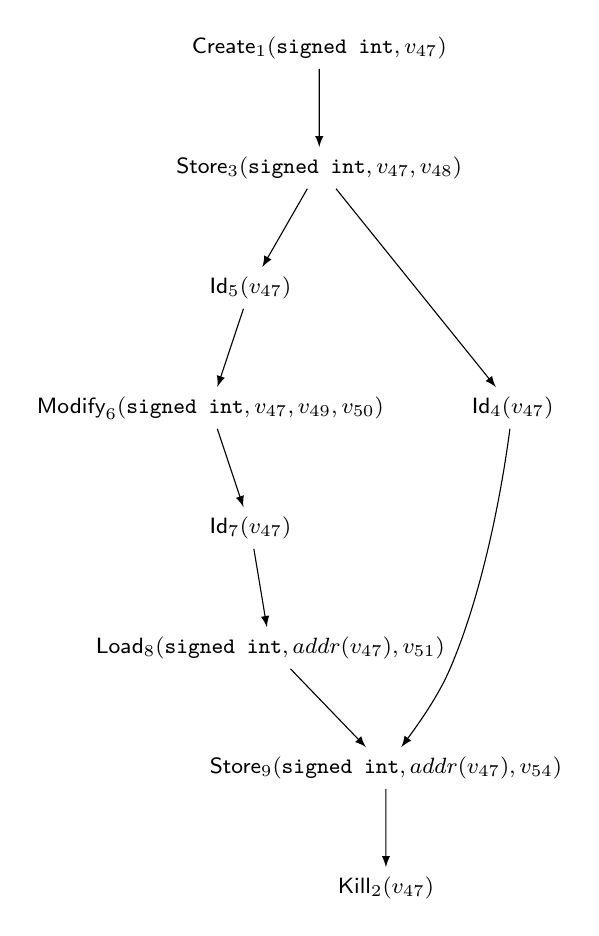
\begin{tikzpicture}[>=latex, scale=0.8]
      \tikzstyle{every node}=[font=\footnotesize]
      %%
\node (v2_9) at (163bp,63bp) [draw,draw=none] {$\tsem{Store}_{9} (\tcc{signed int}, addr (v_{47}), v_{54})$};
  \node (v2_8) at (111bp,117bp) [draw,draw=none] {$\tsem{Load}_{8} (\tcc{signed int}, addr (v_{47}), v_{51})$};
  \node (v2_1) at (133bp,387bp) [draw,draw=none] {$\tsem{Create}_{1} (\tcc{signed int}, v_{47})$};
  \node (v2_3) at (133bp,333bp) [draw,draw=none] {$\tsem{Store}_{3} (\tcc{signed int}, v_{47}, v_{48})$};
  \node (v2_2) at (163bp,9bp) [draw,draw=none] {$\tsem{Kill}_{2} (v_{47})$};
  \node (v2_5) at (102bp,279bp) [draw,draw=none] {$\tsem{Id}_{5} (v_{47})$};
  \node (v2_4) at (220bp,225bp) [draw,draw=none] {$\tsem{Id}_{4} (v_{47})$};
  \node (v2_7) at (102bp,171bp) [draw,draw=none] {$\tsem{Id}_{7} (v_{47})$};
  \node (v2_6) at (84bp,225bp) [draw,draw=none] {$\tsem{Modify}_{6} (\tcc{signed int}, v_{47}, v_{49}, v_{50})$};
  \draw [->] (v2_5) ..controls (96.616bp,262.85bp) and (93.136bp,252.41bp)  .. (v2_6);
  \draw [->] (v2_3) ..controls (154.66bp,306.11bp) and (187.96bp,264.78bp)  .. (v2_4);
  \draw [->] (v2_1) ..controls (133bp,371.01bp) and (133bp,360.86bp)  .. (v2_3);
  \draw [->] (v2_7) ..controls (104.68bp,154.93bp) and (106.39bp,144.64bp)  .. (v2_8);
  \draw [->] (v2_3) ..controls (123.59bp,316.61bp) and (117.34bp,305.72bp)  .. (v2_5);
  \draw [->] (v2_9) ..controls (163bp,47.006bp) and (163bp,36.861bp)  .. (v2_2);
  \draw [->] (v2_6) ..controls (89.384bp,208.85bp) and (92.864bp,198.41bp)  .. (v2_7);
  \draw [->] (v2_8) ..controls (127.16bp,100.22bp) and (138.38bp,88.569bp)  .. (v2_9);
  \draw [->] (v2_4) ..controls (216.35bp,196.72bp) and (208.49bp,146.61bp)  .. (192bp,108bp) .. controls (187.81bp,98.188bp) and (181.55bp,88.127bp)  .. (v2_9);
%

    \end{tikzpicture}
  }
\end{figure}
We choose to follow the definition of the latest draft but since the standard
committee intends to keep the sequencing behaviour unchanged, this change might
be an error in the draft.

\subsection{Memory}
The rules of the previous sections interact with memory by accumulating actions
and ordering constraints but we still have to create an explicit model of memory
in order to determine, for example, the outcome of a particular execution or to
determine whether a program has undefined behaviour.

\subsubsection{Map of values or array of bytes?}
The first decision we have to make concerns what kind of information is stored
in memory. The standard states that each value stored in memory is represented
as a sequence of bytes, which is called \textit{object representation}. A
program can use \lstinline{unsigned char} pointers to examine the object
representation of a value byte-by-byte and therefore our semantics must take
object representations into account. Thus, we could view memory as a map from
addresses to bytes.

Unfortunately, the memory-as-byte-array view has serious
disadvantages. According to the standard, there is no function that relates
values to object representations since a value can have several distinct object
representations. We can only rely on the (implementation-defined) inverse, which
is a surjective function from object representations to values. The lack of a
bijection between the two representations makes the memory-as-byte-array model
impractical.

Our semantics takes an alternative view: memory is represented as map from
symbolic location to values and we only revert to the object representation of a
value when strictly necessary. In comparison, the choice has the drawback that
pointer operations are not quite as straightforward to model as before. However,
most memory operation, e.g. \lstinline{a = 1}, are substantially simplified.

\subsubsection{Enumerating all orderings of memory actions}
Our dynamic semantics describes the meaning of C programs as a collection of
$m$-sets. Each $m$-set corresponds to a distinct path through the program and is
comprised of a set of constraints, a set of memory actions, and the
sequenced-before relation. However, $m$-sets do not directly give us the
information we want. For example, we would like to check whether a program has
undefined behaviour or what the set of possible return values is.

To retrieve this information, we need to symbolically execute the memory actions
and, in turn, complete the constraint set with the information gained from
symbolic execution. Since different orderings of actions potentially lead to
different behaviour, we have to, in general, consider every permutation of
actions that satisfies the sequenced-before relation.

The naive algorithm of generating every permutation and checking whether it is
in accordance with the sequenced-before relation would be very
wasteful. Instead, we exploit a number of observations to arrive at a more
conservative algorithm.
\begin{enumerate}
\item According to the standard, actions of one function call are not allowed to
  overlap with those of another call. Hence, we can consider each function call
  separately.
\item Only the relative ordering of load, store, modify and call actions can
  change the end result, so we do not have to permute any other unsequenced
  actions.
\item If two unsequenced actions cause a data races, behaviour is undefined
  unless they are separated by an indeterminately sequenced function call. Thus,
  when we have a number of load, store, or modify actions that are unsequenced
  with respect to each other (but no such call action), we can choose any
  ordering. We only need to include a constraint expressing that, if any two
  actions, where one is a write or a modify action, operate on the same address,
  then predicate \sem{undef} is true.
\end{enumerate}
These insights almost directly lead to an algorithm that produces the minimal
set of memory orderings that potentially have different behaviour assuming that
we cannot distinguish the memory addresses that the actions operate on, which
often will still be unknown at this point. We omit describing the exact
operation of the algorithm since it is rather technical.

\subsubsection{Executing a trace}
Once all traces that satisfy the sequenced-before relation have been found, we
need to execute each trace. The general process is conceptually fairly
straightforward.

Actions model the interactions of a program with memory. We represent memory as
a partial map from symbolic memory locations to (typed) objects, where an object
can either be a scalar, i.e. containing just one value, or an array of values.

Given a trace and a constraint set, we execute each action of the trace in
order, where our memory is initially just the empty map. If the next action is,
for example, $\sem{Create}_{3}(\cc{int}, s_{2})$, we add a new mapping, $s_2
\mapsto \sem{Scalar}(\cc{int}, \sem{Indet})$, to memory. Note that the value of
the object is initially indeterminate as indicated by the abstract value
\sem{Indet}. If we subsequently encounter a load from address $s_2$ without an
intermediate write, then behaviour is undefined and, thus, we add the predicate
\sem{undef} to the constraint set.

Executing a load action, e.g. $\sem{Load}_{7}(\cc{int}, s_{4}, v_{5})$, is more
involved: First, we have to check whether $s_4$ is a valid memory address. If
not, behaviour is undefined. Otherwise, we retrieve the corresponding object from
memory and verify that type \cc{int} is compatible with the type of the object. If
not, behaviour is undefined. Otherwise, we examine the value $v$ stored in the
object. If it is $\sem{Indet}$, behaviour is undefined. Otherwise, we add $v_5 =
v$ to the constraint set.

Unfortunately, the address, e.g. $s_{4}$, will often not be a symbolic location
but a variable, whose specific value has to be inferred from the constraint
set. We need a constraint solving procedure that allows us to translate
variables to ground terms.

%\subsection{Detecting undefined behaviour}
%infeasible paths unsatisfiable
%A program has undefined behaviour if there is some record $m$ in its $m$-set
%such that $m \wedge \sem{undef}$ is satisfiable.

%\subsubsection{Evaluation order}
%\subsubsection{Sequence points and the sequenced-before relation}
%\subsubsection{Value computation for lvalues}
%\paragraph{Inconsistent use of sequence points}
%\paragraph{Sequencing in initialisers}

\section{Constraint solving}\label{constraintSolving}
We have already seen that equational reasoning is necessary to execute traces.
If we restrict equational logic to ground terms, congruence closure algorithms
give us a complete decision procedures. Congruence closure is most readily
understood by comparison with the union-find problem. A union-find algorithm
maintains an equivalence relation, $\sim$, induced by a list of pairs $(t_i,
s_i)$ such that $t_i \sim s_i$. Similarly, a congruence closure algorithm
maintains a congruence relation $\approx$ induced by a list of pairs $(t_i,
s_i)$ such that $t_i \approx s_i$ satisfying, as before, reflexivity, symmetry,
and transitivity but also the congruence property, i.e.
\begin{equation*}
\inferrule* [Left=\textsc{[congruence]}, Right={.}] {
\Delta \vdash s_1 \approx t_1 \\
\dots \\
\Delta \vdash s_n \approx t_n
} {
\Delta \vdash f (s_1, \dotsc, s_n) \approx f (t_1, \dotsc, t_n)
}
\end{equation*}
For example, given the formula $a = b \wedge f(a) = e \wedge f(b) = d$, a
congruence closure algorithm must be able to infer that $e = d$: By congruence,
$a = b$ implies $f(a) = f(b)$ and transitivity gives us $e = d$.

We implement a modified, persistent version of Nieuwenhuis and Oliveras'
\textquote{fast congruence closure} algorithm \cite{fastCC}, which has best
known time complexity $O(n \log n)$. Our version works on top of a persistent
variant of Tarjan's classic union-find algorithm and uses persistent
arrays. Both are due to Conchon and Filli\^{a}tre \cite{unionFind}. Our
modification has the benefit that it can be easily used within a backtracking
solution procedure.

A congruence closure algorithm alone is only powerful enough to decide
conjunctions of equation but the logic of constraint sets also includes
disjunctions, implications, various integer operations, and integer
comparisons. We could extend the decision procedure to disjunctions and
implications by either translating input formulae into disjunctive normal form
or use a satisfiability solver to perform semantic case splits. Inspection of
our dynamic semantics and the trace execution shows that disjunctions and
implications are only used in constraints describing implementation-defined
behaviour and the occurrence of undefined behaviour. The former involves
implicit universal quantification, for which far more proof power would be
necessary, and the latter is irrelevant for inferring memory addresses. Thus,
there is no need to extend the decision procedure.

We combine the congruence closure algorithm with simple term rewriting
techniques. Using the information collected by the congruence closure algorithm,
we rewrite variables to equivalent ground terms and check equalities and
disequalities. Furthermore, we evaluate constants, e.g. $5 + 2$, and evaluate
predicates, e.g. $4 < 3$, that no longer contain any variables. We also have
specialised rules that remove unnecessary comparisons due to type conversions
and overflow checks, e.g. $i \leq \cc{INT\_MAX}$, when $i$ is known to be
smaller than or equal to minimal value of $\cc{INT\_MAX}$ allowed by the
standard.

In practice, our approach turns out to be powerful enough to tackle all tested
programs free of implementation-defined behaviour. It is not clear how one
should proceed with implementation-defined programs: We choose to return a
partially evaluated $m$-set if constraint solving fails. Another approach would
be to encode trace execution in a more powerful logic but the benefits are not
obvious.

\section{Software design}
Throughout the implementation chapter we have presented the workings of our tool
in the form of simplified and stylised inference rules. In this last section we
give an overview of the tool design and demonstrate how closely our code
corresponds to the typeset rules.

The general structure is very similar to a compiler pipeline. In fact, the first
few phases of our tool are commonly found in compilers: lexing, parsing, scope
analysis and identifier disambiguation, removal of syntactic sugar, translation
to a common intermediate language, and type checking and annotating the AST with
type information. The subsequent phases, the semantic analysis, enumeration of
all traces of memory action, and constraint solving, are, however, highly
non-standard. The reason is that our target language of $m$-sets bears little
resemblance to the machine languages compilers usually generate.

Above we speak of a pipeline structure because each phase is, in abstract terms,
a function from some type $t_i$ to $t_{i+1}$ and the next a function from
$t_{i+1}$ to $t_{i+2}$, etc. Thus, at the highest level of code, we use the
\textit{pipeline} function \cite[p. 45]{expertFS}
%\begin{figure}[htb]
\begin{lstlisting}[language=ML, frame=none]
    let (|>) x f = f x : 'a -> ('a -> 'b) -> 'b
\end{lstlisting}
%\end{figure}
to combine the different phases, i.e.
\begin{lstlisting}[language=ML]
...
      file_name
      |> Input.from_file
      |> Lexer.make
      |> Parser.parse
      |> CabsToAil.desugar "main"
      |> AilTyping.annotate
      ...
\end{lstlisting}

Each such phase is contained in a separate module. We followed the principle
that a each module should only implement a single task. To enforce this
separation of concerns, we made extensive use of module signatures and abstract
types to seal the module definition and to prevent implementation details of the
module leaking into unrelated code.

In the following we focus on the type-checking and semantic analysis phases. For
each, we show code excerpts and put them in relation to rules presented earlier.

Function \lstinline[language=ML]{check_exp} in Fig. \ref{codeTypeChecking}
computes the type of a given expression \lstinline[language=ML]{exp} whose
subexpressions have already been annotated with types. The excerpt implements
the \textsc{[indir-pointer]} and \textsc{[indir-function]} rules from section
\ref{typeChecking}. Since the indirection operator expects a non-lvalue, the
inlined lvalue conversion rule (c.f. inference rule \textsc{[lvalue-conv]}) is
applied to operand $e$ as part of function \lstinline[language=ML]{f}: The
function retrieves the type annotation (\lstinline[language=ML]{AA.type_of}),
performs, if necessary, lvalue conversion
(\lstinline[language=ML]{AT.lvalue_convert}), and turns array and function types
into pointer types (\lstinline[language=ML]{AT.pointer_convert}).
\begin{figure}[htb]
\begin{lstlisting}[language=ML,frame=tblr]
let rec check_exp env exp =
  ...
  let f e =
    let t = match AA.type_of e with
      | A.Exp    t -> t
      | A.Lvalue t -> AT.lvalue_convert t in
    AT.pointer_convert t in
  ...
  match exp with
  ...
  | A.UNARY (A.INDIRECTION, e) ->
      let msg = "Violation of constraint 6.5.3.2 #2 Address and indirection \
                 operators, Constraints: \'The operand of the unary * \
                 operator shall have pointer type.\'" in
      let t = f e in
      if AT.is_pointer t then
        if AT.is_pointer_to_object t then
          A.Lvalue (AT.base_of_pointer t)
        else A.Exp (AT.base_of_pointer t)
      else invalid msg
  ...
\end{lstlisting}
\caption{Type-checking expression $\cc{*}e$}\label{codeTypeChecking}
\end{figure}
If the type of $e$ after appropriate conversions is a not a pointer type, the
expression is ill-typed and we produce an error message quoting the
corresponding paragraph from the standard. Otherwise we make sure to return an
expression type instead of an lvalue type if the operand is a function.

The code implementing the dynamic semantics is even closer to the typeset
version. The OCaml datatype below is practically identical to the record type
\sem{meaning} given in Section \ref{generalForm}.
\begin{figure}[htb]
\begin{lstlisting}[language=ML, frame=tblr]
type meaning = {
  actions : action Set.t;
  seq_before : (action * action) Set.t;
  fs_actions : (action, action Set.t) Map.t;
  constraints : AC.t
}
\end{lstlisting}
\caption{The OCaml record type corresponding to \sem{meaning} defined in Section \ref{generalForm}}
\end{figure}

Similarly, our code uses the same set-based operations to combine such records,
e.g. Fig. \ref{codeSbAnd} is the OCaml equivalent of the $\sband$ operator.
\begin{figure}[htb]
\begin{lstlisting}[language=ML, frame=tblr]
let and_meanings_sb m1 m2 = {
  actions = Set.union m1.actions m2.actions;
  seq_before =
    begin
      let sb = Set.product m1.actions m2.actions in
      Set.union sb (Set.union m1.seq_before m2.seq_before)
    end;
  fs_actions = Map.union m1.fs_actions m2.fs_actions;
  constraints = AC.union m1.constraints m2.constraints
}
\end{lstlisting}
\caption{Implementation of $m_1 \protect\sband m_2$, where
  \lstinline[language=ML]{Set.product} is the Cartesian product}
\label{codeSbAnd}
\end{figure}
The only difference lies in the representation of constraints: In the typeset
version the conjunction of two logical formulae is a purely syntactic operation
but our code must use an explicit data structure, namely sets.

Our last code sample, Fig. \ref{codeAdd}, implements rule \textsc{add}:
\lstinline[language=ML]{reduce_exp} is the equivalent of $\denott{e}{\tau}$,
where the function argument \lstinline[language=ML]{env} corresponds to
$\Sigma$.
\begin{figure}[hbt]
\begin{lstlisting}[language=ML, frame=tblr]
and reduce_exp env file exp =
  ...
  let conv e = ATC.conv (AA.exp_type_of exp) (reduce_exp env file e) in
  ...
  match AA.exp_of exp with
  ...
  | A.BINARY (Cabs.ARITHMETIC Cabs.ADD, e1, e2)
      when AT.is_arithmetic (AA.exp_type_of e1)
        && AT.is_arithmetic (AA.exp_type_of e2)
        && AT.is_signed_integer(AA.exp_type_of exp) ->
      let a1, m1 = conv e1 in
      let a2, m2 = conv e2 in
      let a = AC.fresh_name () in
      let sum = AC.eq a (AC.plus a1 a2) in
      let overflow =
        AC.implies
          (AC.neg (ATC.in_range (AA.exp_type_of exp) a))
          AC.undef in
      a, m1 <&> m2 <&- sum <&- overflow
\end{lstlisting}
\caption{The dynamic semantics of $e_1 \cc{+} e_2$ (c.f. rule \textsc{[add]} in
  Section \ref{arithmetic})}
\label{codeAdd}
\end{figure}
The typed-related premises of rule \textsc{[add]} are translated to pattern
matching guards (e.g. \lstinline[language=ML]{when AT.is_arithmetic ...}). And
the inductive premises on expressions \lstinline[language=ML]{e1} and
\lstinline[language=ML]{e2} are expressed by function
\lstinline[language=ML]{conv}, which also implements the necessary type
conversions. The main thing to notice is, however, how close the resulting value
of the function, \lstinline[language=ML]{a, m1 <&> m2 <&- sum <&- overflow}
(where \lstinline[language=ML]{<&>} stands for $\otimes$ and
\lstinline[language=ML]{<&-} for $\wedge$), is to that of the inference rule.

To give an idea of the size of the implementation, we conclude the chapter with
a few rough source line counts (excluding signature files): Parsing required
about 1000, translation into abstract syntax 500, type checking 1000, semantic
analysis 1500, and constraint solving 750 lines of OCaml code. Additionally,
around 500 lines of source code are shared between the individual modules.

% Evaluation + Conclusion: 2300 words.
\chapter{Evaluation}
In this chapter, we examine how the tool stacks up against the success criteria
of our project proposal and analyse its capabilities and limitations and also
take a look at its performance using a range of selected programs.

The fundamental problem with evaluating a project whose principal goal it is to
demonstrate that C can be fully formalised, is lack of a litmus test: We obtain
a formal definition from interpreting the standard which sometimes, as we have
seen in the previous chapter, involves making unverifiable choices that will not
be universally accepted. The best we can do is to compare our interpretation
with those of others. Specifically, we compare against the results produced by
compilers for programs that exhibit interesting behaviour.

\section{Success criteria}
The original proposal declared that, to be deemed successful, our project would
have to satisfy the following two requirements.

\begin{enumerate}
\item\label{sc1} The tool accepts C programs restricted to integer expressions
  and generates graphs presenting the standard-conforming traces.
\item\label{sc2} For relevant programs from GCC's C test suite, the set of
  results produced by the tool subsumes the behaviour of the compiled
  program. Any discrepancy must be explained.
\end{enumerate}

As we will see later, our tool goes far beyond what the first half of Criterion
\ref{sc1} demands: It parses C programs, detects ill-typed programs and is able
to produce meaningful result for not just integer expressions but also for
programs with pointers, pointer arithmetic, fixed-length arrays, (recursive)
function calls, and loops containing continue and break statements. All of these
features were implemented on top of what the proposal required giving a far more
complete picture of C than originally planned.

The second half of Criterion \ref{sc1} is also met: The various graphs in the
following sections visualising the sequenced-before relation have been
automatically generated by our tool.

Criterion \ref{sc2} demands that we test our tool on C programs selected from
GCC's C language test suite. The test suite is comprised of a large number of
regression tests. Most of them test GCC-specific features that are not part of
the standard, compiler flags, or platform-specific miscompilations. As the test
suite contains very few relevant as well as interesting programs, we mainly used
test programs due to John Regehr, whose work on automated testing of C compilers
has revealed hundreds of compiler bugs \cite{regehr}. These programs are
particularly interesting since some compilers do get them wrong.

\section{Capabilities}
We begin with the following program.  \lstinputlisting{examples/ptr_regehr.c} It
is taken straight from a blog entry by John Regehr\footnote{J. Regehr,
  \textit{An Executable Semantics For C Is Useful},
  \url{http://blog.regehr.org/archives/523}.} on the potential benefits of an
executable semantics for C. The program has a whole range of possible sources of
undefined behaviour: The pointers \cc{p1} and \cc{p2} must both be valid and
correctly aligned, the result of \cc{*p2} must not be zero, the increment
operators must not produce overflows, and \cc{p1} and \cc{p2} must point to
disjoint memory regions. Otherwise behaviour is undefined.

The last condition in the list is not immediately obvious and requires more
explanation. Consider the graph Fig. \ref{ptrRegehrFoo} generated by our
tool. It shows the sequenced-before relation on memory actions in function
\cc{foo}. An execution of the function is allowed to choose any order of side
effects that satisfies the sequenced-before relation. In particular, the two
modify actions, $15$ and $19$, can appear in either order, since they are
unsequenced. It follows from the discussions of the previous chapter that
behaviour is undefined if both actions operate on the same address, i.e. $v_{52}
= v_{56}$.
\begin{figure}[htb]
\centering
  \fbox{
    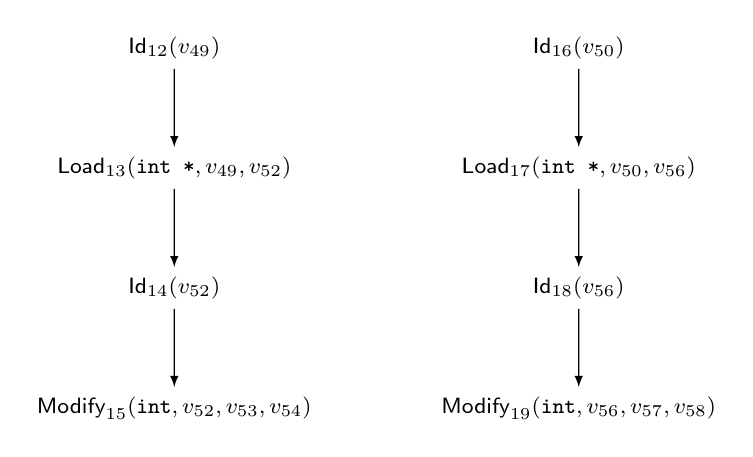
\begin{tikzpicture}[>=latex, scale=.8]
      \tikzstyle{every node}=[font=\footnotesize]
      %%
\node (v2_13) at (82bp,117bp) [draw,draw=none] {$\tsem{Load}_{13} (\tcc{int *}, v_{49}, v_{52})$};
  \node (v2_12) at (82bp,171bp) [draw,draw=none] {$\tsem{Id}_{12} (v_{49})$};
  \node (v2_15) at (82bp,9bp) [draw,draw=none] {$\tsem{Modify}_{15} (\tcc{int}, v_{52}, v_{53}, v_{54})$};
  \node (v2_14) at (82bp,63bp) [draw,draw=none] {$\tsem{Id}_{14} (v_{52})$};
  \node (v2_17) at (264bp,117bp) [draw,draw=none] {$\tsem{Load}_{17} (\tcc{int *}, v_{50}, v_{56})$};
  \node (v2_16) at (264bp,171bp) [draw,draw=none] {$\tsem{Id}_{16} (v_{50})$};
  \node (v2_19) at (264bp,9bp) [draw,draw=none] {$\tsem{Modify}_{19} (\tcc{int}, v_{56}, v_{57}, v_{58})$};
  \node (v2_18) at (264bp,63bp) [draw,draw=none] {$\tsem{Id}_{18} (v_{56})$};
  \draw [->] (v2_14) ..controls (82bp,47.006bp) and (82bp,36.861bp)  .. (v2_15);
  \draw [->] (v2_18) ..controls (264bp,47.006bp) and (264bp,36.861bp)  .. (v2_19);
  \draw [->] (v2_12) ..controls (82bp,155.01bp) and (82bp,144.86bp)  .. (v2_13);
  \draw [->] (v2_13) ..controls (82bp,101.01bp) and (82bp,90.861bp)  .. (v2_14);
  \draw [->] (v2_16) ..controls (264bp,155.01bp) and (264bp,144.86bp)  .. (v2_17);
  \draw [->] (v2_17) ..controls (264bp,101.01bp) and (264bp,90.861bp)  .. (v2_18);
%

    \end{tikzpicture}
  }
\caption{Ordering of actions in function \cc{foo}}
\label{ptrRegehrFoo}
\end{figure}

Our algorithm enumerating action traces detects that the modify actions are
unsequenced and therefore adds a constraint
\begin{equation*}
v_{52} = v_{56} \rightarrow \sem{undef}
\end{equation*}
to the set of constraints. Later, when each trace is (symbolically) executed,
the tool (c.f. store actions $6$ and $9$ in \ref{ptrRegehrMain}) stores the
symbolic address $v_{47}$ in the memory locations $v_{49}$ and $v_{50}$ for the
function arguments \cc{p1} and \cc{p2}, respectively. Subsequently, function
\cc{foo} retrieves the value of each argument from memory (load actions $13$ and
$17$) yielding two further constraints: $v_{52} = v_{47}$ and $v_{56} =
v_{47}$. The congruence closure algorithm is then able to infer that, by
transitivity, we also must have $v_{52} = v_{56}$. Finally, our constraint
simplification algorithm uses the new information to rewrite the
constraint
\begin{equation*}
v_{52} = v_{56} \rightarrow \sem{undef}
\end{equation*}
to $\sem{undef}$.
\begin{figure}[htb]
\centering
  \fbox{
    \begin{tikzpicture}[>=latex, scale=.8]
      \tikzstyle{every node}=[font=\footnotesize]
      
%%
\node (v2_11) at (216bp,63bp) [draw,draw=none] {$\tsem{Kill}_{11} (v_{50})$};
  \node (v2_10) at (310bp,63bp) [draw,draw=none] {$\tsem{Kill}_{10} (v_{49})$};
  \node (v2_20) at (263bp,115bp) [draw,draw=none] {$\tsem{Call}_{20} $};
  \node (v2_9) at (159bp,167bp) [draw,draw=none] {$\tsem{Store}_{9} (\tcc{int *}, v_{50}, v_{47})$};
  \node (v2_8) at (74bp,221bp) [draw,draw=none] {$\tsem{Create}_{8} (\tcc{int *}, v_{50})$};
  \node (v2_1) at (263bp,329bp) [draw,draw=none] {$\tsem{Create}_{1} (\tcc{signed int}, v_{47})$};
  \node (v2_3) at (263bp,275bp) [draw,draw=none] {$\tsem{Store}_{3} (\tcc{signed int}, v_{47}, v_{48})$};
  \node (v2_2) at (263bp,9bp) [draw,draw=none] {$\tsem{Kill}_{2} (v_{47})$};
  \node (v2_5) at (326bp,221bp) [draw,draw=none] {$\tsem{Create}_{5} (\tcc{int *}, v_{49})$};
  \node (v2_4) at (452bp,221bp) [draw,draw=none] {$\tsem{Id}_{4} (v_{47})$};
  \node (v2_7) at (200bp,221bp) [draw,draw=none] {$\tsem{Id}_{7} (v_{47})$};
  \node (v2_6) at (367bp,167bp) [draw,draw=none] {$\tsem{Store}_{6} (\tcc{int *}, v_{49}, v_{47})$};
  \draw [->] (v2_4) ..controls (425.08bp,203.9bp) and (404.73bp,190.97bp)  .. (v2_6);
  \draw [->] (v2_11) ..controls (230.54bp,46.298bp) and (240.54bp,34.801bp)  .. (v2_2);
  \draw [->] (v2_20) ..controls (249.76bp,100.36bp) and (239.13bp,88.586bp)  .. (v2_11);
  \draw [->] (v2_6) ..controls (332.45bp,149.73bp) and (305.48bp,136.24bp)  .. (v2_20);
  \draw [->] (v2_20) ..controls (276.24bp,100.36bp) and (286.87bp,88.586bp)  .. (v2_10);
  \draw [->] (v2_3) ..controls (325.16bp,257.24bp) and (376.53bp,242.56bp)  .. (v2_4);
  \draw [->] (v2_10) ..controls (295.46bp,46.298bp) and (285.46bp,34.801bp)  .. (v2_2);
  \draw [->] (v2_5) ..controls (338.56bp,204.46bp) and (347.06bp,193.26bp)  .. (v2_6);
  \draw [->] (v2_9) ..controls (193.55bp,149.73bp) and (220.52bp,136.24bp)  .. (v2_20);
  \draw [->] (v2_3) ..controls (282.53bp,258.26bp) and (296.74bp,246.08bp)  .. (v2_5);
  \draw [->] (v2_1) ..controls (263bp,313.01bp) and (263bp,302.86bp)  .. (v2_3);
  \draw [->] (v2_3) ..controls (243.47bp,258.26bp) and (229.26bp,246.08bp)  .. (v2_7);
  \draw [->] (v2_7) ..controls (187.44bp,204.46bp) and (178.94bp,193.26bp)  .. (v2_9);
  \draw [->] (v2_3) ..controls (200.84bp,257.24bp) and (149.47bp,242.56bp)  .. (v2_8);
  \draw [->] (v2_8) ..controls (100.92bp,203.9bp) and (121.27bp,190.97bp)  .. (v2_9);
%

    \end{tikzpicture}
  }
\caption{Ordering of actions in function \cc{main}}
\label{ptrRegehrMain}
\end{figure}

Since the constraint set is still satisfiable after all actions have been
executed, i.e. the set does not correspond to an infeasible path, we can
conclude that the program has undefined behaviour. After the process described
above, our tool therefore outputs the following fully simplified constraint set:
\begin{lstlisting}
/\ {
  UNDEFINED = 1,
  v1_48 = 1,
  v1_52 = addr (v1_47),
  v1_53 = 1,
  v1_54 = 2,
  v1_55 = 1,
  v1_56 = addr (v1_47),
  v1_57 = v1_54,
  v1_58 = 3,
  v1_59 = 2,
  v1_60 = v1_51,
  v1_60 = 1,
  v1_61 = return,
  v1_61 = 1
}
\end{lstlisting}

Even though the program is very small, the analysis necessary to reliably detect
the unsequenced race that results in undefined behaviour is surprisingly
involved. Which may also be why \textquote{very few tools for analyzing C code
  find this error} as Regehr remarks referring to his example program.

Next, we briefly look at two variations of the above program
demonstrating that our tools models C's underspecified evaluation order
correctly. The first programs splits the increment operations into separate
function calls but otherwise preforms the same work.
\lstinputlisting{examples/ptr_fg.c}

Indeed, the ordering of memory events in function \cc{main} (see
Fig. \ref{ptrFgMain}) is almost exactly the same as before. The only difference
is the additional call action which is unsequenced with respect to the other
call action.
\begin{figure}[htb]
\centering
  \fbox{
    \begin{tikzpicture}[>=latex, scale=.8]
      \tikzstyle{every node}=[font=\footnotesize]
      %%
\node (v2_13) at (206bp,221bp) [draw,draw=none] {$\tsem{Id}_{13} (v_{47})$};
  \node (v2_12) at (367bp,115bp) [draw,draw=none] {$\tsem{Call}_{12} $};
  \node (v2_15) at (165bp,167bp) [draw,draw=none] {$\tsem{Store}_{15} (\tcc{int *}, v_{56}, v_{47})$};
  \node (v2_14) at (76bp,221bp) [draw,draw=none] {$\tsem{Create}_{14} (\tcc{int *}, v_{56})$};
  \node (v2_16) at (239bp,63bp) [draw,draw=none] {$\tsem{Kill}_{16} (v_{56})$};
  \node (v2_21) at (224bp,115bp) [draw,draw=none] {$\tsem{Call}_{21} $};
  \node (v2_1) at (270bp,329bp) [draw,draw=none] {$\tsem{Create}_{1} (\tcc{signed int}, v_{47})$};
  \node (v2_3) at (270bp,275bp) [draw,draw=none] {$\tsem{Store}_{3} (\tcc{signed int}, v_{47}, v_{48})$};
  \node (v2_2) at (288bp,9bp) [draw,draw=none] {$\tsem{Kill}_{2} (v_{47})$};
  \node (v2_5) at (334bp,221bp) [draw,draw=none] {$\tsem{Create}_{5} (\tcc{int *}, v_{49})$};
  \node (v2_4) at (460bp,221bp) [draw,draw=none] {$\tsem{Id}_{4} (v_{47})$};
  \node (v2_7) at (338bp,63bp) [draw,draw=none] {$\tsem{Kill}_{7} (v_{49})$};
  \node (v2_6) at (375bp,167bp) [draw,draw=none] {$\tsem{Store}_{6} (\tcc{int *}, v_{49}, v_{47})$};
  \draw [->] (v2_7) ..controls (322.54bp,46.298bp) and (311.89bp,34.801bp)  .. (v2_2);
  \draw [->] (v2_14) ..controls (104.18bp,203.9bp) and (125.49bp,190.97bp)  .. (v2_15);
  \draw [->] (v2_15) ..controls (183.83bp,150.4bp) and (197.56bp,138.31bp)  .. (v2_21);
  \draw [->] (v2_16) ..controls (254.16bp,46.298bp) and (264.59bp,34.801bp)  .. (v2_2);
  \draw [->] (v2_3) ..controls (332.63bp,257.2bp) and (384.58bp,242.44bp)  .. (v2_4);
  \draw [->] (v2_4) ..controls (433.08bp,203.9bp) and (412.73bp,190.97bp)  .. (v2_6);
  \draw [->] (v2_5) ..controls (346.56bp,204.46bp) and (355.06bp,193.26bp)  .. (v2_6);
  \draw [->] (v2_12) ..controls (359.04bp,100.73bp) and (352.92bp,89.752bp)  .. (v2_7);
  \draw [->] (v2_3) ..controls (250.16bp,258.26bp) and (235.72bp,246.08bp)  .. (v2_13);
  \draw [->] (v2_1) ..controls (270bp,313.01bp) and (270bp,302.86bp)  .. (v2_3);
  \draw [->] (v2_3) ..controls (206.06bp,257.2bp) and (153.01bp,242.44bp)  .. (v2_14);
  \draw [->] (v2_6) ..controls (372.58bp,151.27bp) and (370.98bp,140.89bp)  .. (v2_12);
  \draw [->] (v2_13) ..controls (193.44bp,204.46bp) and (184.94bp,193.26bp)  .. (v2_15);
  \draw [->] (v2_3) ..controls (289.84bp,258.26bp) and (304.28bp,246.08bp)  .. (v2_5);
  \draw [->] (v2_21) ..controls (228.05bp,100.95bp) and (231.08bp,90.441bp)  .. (v2_16);
%

    \end{tikzpicture}
  }
\caption{Sequenced-before relation for actions in function \cc{main}}
\label{ptrFgMain}
\end{figure}
Since each function call contains a modify action on the location of \cc{x}, one
might naively expect this program also to have undefined behaviour but, as
discussed before, the standard states that the actions of a function call are
indeterminately sequenced with respect to the actions of the
callee\footnote{Actions of one function cannot not overlap with those of another
  function.}. In other words, the two modify actions are not unsequenced, they
can be executed in any order and behaviour is still defined. Correspondingly,
our tool indicates that the program is free of undefined behaviour.
\begin{lstlisting}
/\ {
  ...
  v1_51 = addr (v1_47),
  ...
  v1_58 = addr (v1_47),
  ...
  v1_63 = return,
  v1_63 = 0
}
\end{lstlisting}
Furthermore, due to the sequenced data race the tool detects a second distinct,
well-defined behaviour for the program with return value one instead zero.
\begin{lstlisting}
/\ {
  ...
  v1_51 = addr (v1_47),
  ...
  v1_58 = addr (v1_47),
  ...
  v1_63 = return,
  v1_63 = 1
}
\end{lstlisting}

The second variant of Regehr's program only moves one of the
increment operators into a function call.  \lstinputlisting{examples/ptr_f.c}

As before, the actions of the call to function \cc{f} are indeterminately
sequenced with respect to the actions occurring in the main function. However,
the increment operator gets special treatment: An implementation is not allowed
to split the load and store actions associated with an increment across a
function call. We should observe exactly two distinct return values identical to
those of the previous program. Our tool produces the simplified constraint
\begin{lstlisting}
/\ {
  ...
  v1_61 = return,
  v1_61 = 0
}
\end{lstlisting}
and
\begin{lstlisting}
/\ {
  ...
  v1_61 = return,
  v1_61 = 1
}
\end{lstlisting}
and, hence, fulfils the rules of the standard.

As a last demonstration, we look at a program with pointer arithmetic. Namely,
the example from Section \ref{pointerArithmetic}.
\lstinputlisting{examples/onebeforemod.c} When fed into our tool, it returns the
following constraint set indicating undefined behaviour.
\begin{lstlisting}
/\{
  true,
  UNDEFINED = 1
  ...
}
\end{lstlisting}
If we modify the program to iterate through the array in the other direction,
behaviour is no longer undefined.  \lstinputlisting{examples/oneafter.c}
Correspondingly, our tool declares that the sum of the array, six, is returned:
\begin{lstlisting}
/\{
  true,
  ...,
  v1_102 = return,
  v1_102 = 6,
  ...
}
\end{lstlisting}

In summary, we have demonstrated that our tool meets our original goals and
more. It faithfully models evaluation order, it can successfully detect
undefined behaviour, and the constraint solving and simplification phase is
powerful enough to solve the constraint sets for many programs. Moreover,
despite written with clarity and correctness in mind rather than performance,
the tool is fast enough for small programs. The tool takes less than a second
for most of programs discussed above.

\section{Limitations}
We have already mentioned one factor that limits our tool: Most real-world
programs are not written in standard-conform C. Like GCC, all major C compilers
support features that are not part of the languages standard and therefore not
supported by our tool.

The other issue we have to worry about is performance. Whilst our tool is
demonstrably fast enough to process a typical GCC test suite program, which was
our main goal, its performance does not scale very well with an increasing
number of case splits. As an illustration consider the following GCC test
computing Fibonacci numbers.  \lstinputlisting{examples/gcc_fib.c}

Each \sem{if} statement causes our tool to perform a case split, i.e. the number
of $m$-sets is doubled. Hence, if $n$ is the recursive call depth, then the
number of $m$-sets generated by our tool will be $2 a(n)$, where $a(k+1) = a(k)^2 + 1$ and $a (0) = 0$. When the above program is fed into our tool, it will
correctly determine that all $m$-sets correspond to infeasible paths for $n \leq
4$ and that exactly one $m$-set is satisfiable for larger $n$. However, the time
it takes to return an answer increases very quickly: For for a call depth $n
\leq 3$ the tool responds within a few seconds but for $n = 5$ it already takes
several hours.

Since the above implementation of the Fibonacci function has exponential time
complexity, we should, of course, also expect to see an exponential increase in
the tool run time but the situation is worsened by the strict separation of
constraint generation and constraint solving: For $n = 5$, the semantic analysis
phase of the tool produces $2a(5) = 1534$ distinct $m$-sets. Each $m$-set is
then evaluated separately. However, we know that the execution paths from which
the individual $m$-sets have been generated, have a large overlap. We could
exploit this knowledge by memoizing and reusing partial evaluations of
$m$-sets. We decided against this optimisation to keep the semantic analysis
clean. As a compromise, we chose to use persistent data structures in the
constraint solving algorithm such that a backtracking strategy can be integrated
at later stage without destroying the software structure of the implementation.

However, the number of $m$-sets alone cannot explain the long running times. If
we modify the program slightly by introducing two temporary variables \cc{x} and
\cc{y} that store the intermediate results of the recursive calls, our tool
needs less than two minutes to spit out a result even though the number of case
splits due to diverging execution paths is unchanged.
\lstinputlisting{examples/fibmod.c}

The discrepancy in run times is best explained with reference to the ordering of
actions in function \cc{fib}. The following graph shows the sequenced-before
relation for the original program.
\begin{figure}[htb]
\centering
  \fbox{
    \begin{tikzpicture}[>=latex, scale=.8]
      \tikzstyle{every node}=[font=\footnotesize]
      %%
\node (v2_10) at (395bp,9bp) [draw,draw=none] {$\tsem{Kill}_{10} (v_{55})$};
  \node (v2_13) at (395bp,61bp) [draw,draw=none] {$\tsem{Call}_{13} $};
  \node (v2_15) at (228bp,167bp) [draw,draw=none] {$\tsem{Load}_{15} (\tcc{int}, v_{47}, v_{73})$};
  \node (v2_14) at (218bp,221bp) [draw,draw=none] {$\tsem{Id}_{14} (v_{47})$};
  \node (v2_17) at (176bp,113bp) [draw,draw=none] {$\tsem{Store}_{17} (\tcc{int}, v_{72}, v_{76})$};
  \node (v2_16) at (68bp,167bp) [draw,draw=none] {$\tsem{Create}_{16} (\tcc{int}, v_{72})$};
  \node (v2_21) at (176bp,61bp) [draw,draw=none] {$\tsem{Call}_{21} $};
  \node (v2_9) at (395bp,113bp) [draw,draw=none] {$\tsem{Store}_{9} (\tcc{int}, v_{55}, v_{59})$};
  \node (v2_8) at (338bp,221bp) [draw,draw=none] {$\tsem{Create}_{8} (\tcc{int}, v_{55})$};
  \node (v2_18) at (176bp,9bp) [draw,draw=none] {$\tsem{Kill}_{18} (v_{72})$};
  \node (v2_5) at (278bp,275bp) [draw,draw=none] {$\tsem{Load}_{5} (\tcc{int}, v_{47}, v_{50})$};
  \node (v2_4) at (278bp,329bp) [draw,draw=none] {$\tsem{Id}_{4} (v_{47})$};
  \node (v2_7) at (447bp,167bp) [draw,draw=none] {$\tsem{Load}_{7} (\tcc{int}, v_{47}, v_{56})$};
  \node (v2_6) at (456bp,221bp) [draw,draw=none] {$\tsem{Id}_{6} (v_{47})$};
  \draw [->] (v2_5) ..controls (259.49bp,258.34bp) and (246.13bp,246.31bp)  .. (v2_14);
  \draw [->] (v2_14) ..controls (220.98bp,204.93bp) and (222.88bp,194.64bp)  .. (v2_15);
  \draw [->] (v2_5) ..controls (296.51bp,258.34bp) and (309.87bp,246.31bp)  .. (v2_8);
  \draw [->] (v2_15) ..controls (211.84bp,150.22bp) and (200.62bp,138.57bp)  .. (v2_17);
  \draw [->] (v2_16) ..controls (102.67bp,149.66bp) and (129.52bp,136.24bp)  .. (v2_17);
  \draw [->] (v2_4) ..controls (278bp,313.01bp) and (278bp,302.86bp)  .. (v2_5);
  \draw [->] (v2_17) ..controls (176bp,97.353bp) and (176bp,87.122bp)  .. (v2_21);
  \draw [->] (v2_13) ..controls (395bp,47.024bp) and (395bp,36.669bp)  .. (v2_10);
  \draw [->] (v2_21) ..controls (176bp,47.024bp) and (176bp,36.669bp)  .. (v2_18);
  \draw [->] (v2_5) ..controls (233.93bp,257.89bp) and (200.72bp,244.18bp)  .. (173bp,230bp) .. controls (143.16bp,214.74bp) and (110.25bp,194.38bp)  .. (v2_16);
  \draw [->] (v2_7) ..controls (430.84bp,150.22bp) and (419.62bp,138.57bp)  .. (v2_9);
  \draw [->] (v2_5) ..controls (336.41bp,257.28bp) and (384.51bp,242.69bp)  .. (v2_6);
  \draw [->] (v2_9) ..controls (395bp,97.353bp) and (395bp,87.122bp)  .. (v2_13);
  \draw [->] (v2_8) ..controls (346.29bp,199.88bp) and (355.87bp,176.74bp)  .. (366bp,158bp) .. controls (371.14bp,148.49bp) and (377.59bp,138.34bp)  .. (v2_9);
  \draw [->] (v2_6) ..controls (453.32bp,204.93bp) and (451.61bp,194.64bp)  .. (v2_7);
%

    \end{tikzpicture}
  }
\caption{Sequenced-before relation for actions in function \cc{fib}}
\label{fibFib}
\end{figure}
Note that the two recursive calls, represented by actions $\sem{Call}_{21}$ and
$\sem{Call}_{13}$, are unsequenced. Recalling the trace enumeration algorithm,
our tool executes both orderings of the two actions. Hence, each recursive call
doubles the number of traces.

In comparison, the call actions of the modified program, $\sem{Call}_{27}$ and
$\sem{Call}_{46}$ in Fig. \ref{fibModFib}, are related: $\sem{Call}_{27}$ is
sequenced before $\sem{Call}_{46}$. Thus, only one trace needs to be executed.
\begin{figure}[htb]
\centering
  \fbox{
    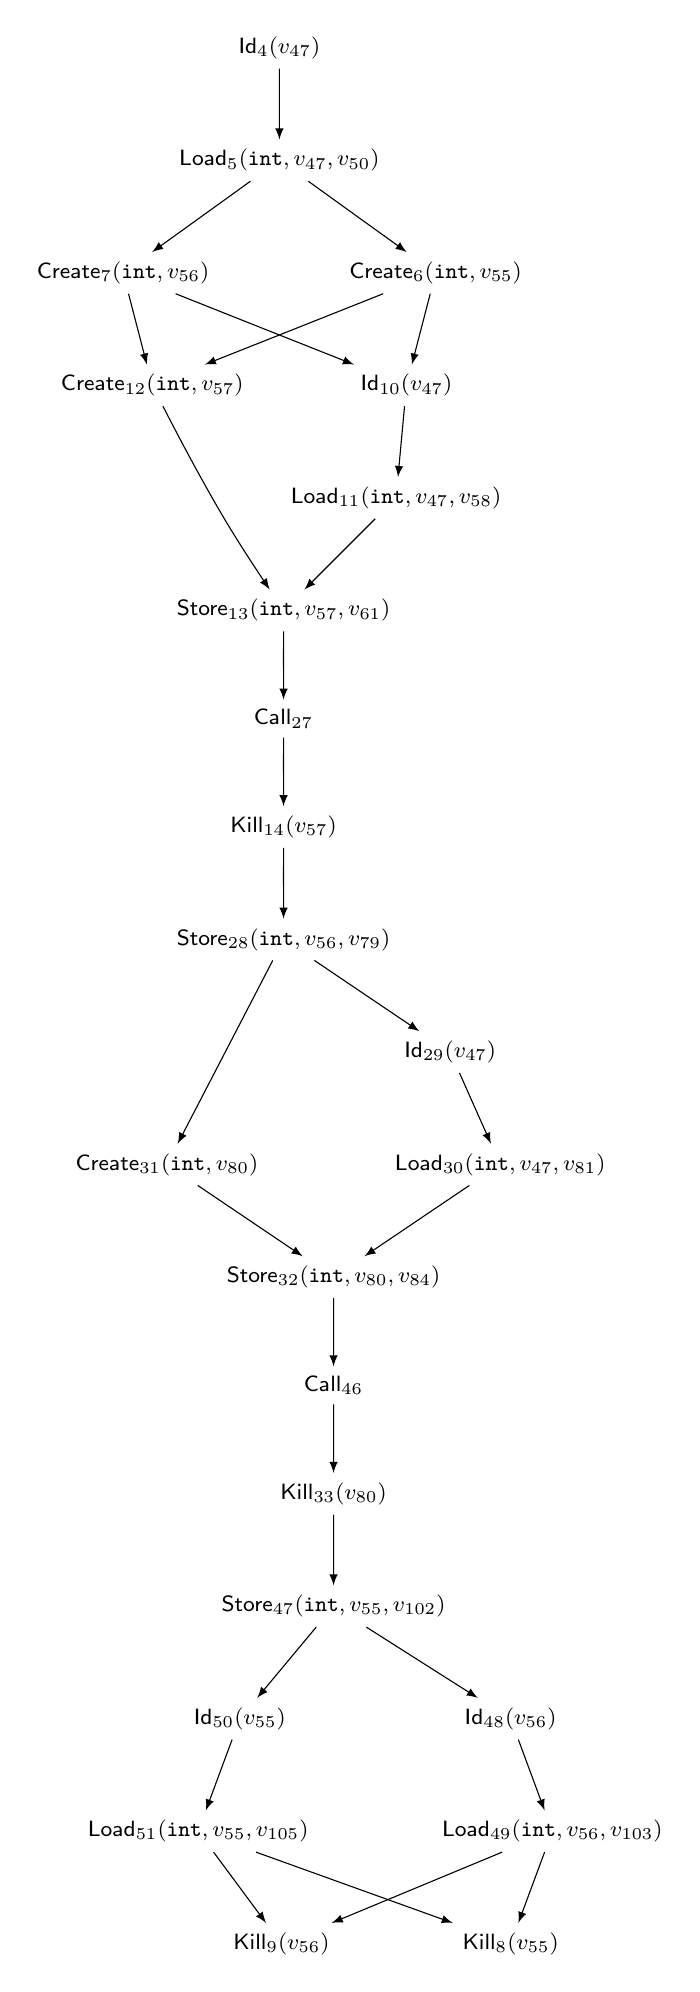
\begin{tikzpicture}[>=latex, scale=.75]
      \tikzstyle{every node}=[font=\footnotesize]
      %%
\node (v2_28) at (143bp,491bp) [draw,draw=none] {$\tsem{Store}_{28} (\tcc{int}, v_{56}, v_{79})$};
  \node (v2_29) at (223bp,437bp) [draw,draw=none] {$\tsem{Id}_{29} (v_{47})$};
  \node (v2_27) at (143bp,597bp) [draw,draw=none] {$\tsem{Call}_{27} $};
  \node (v2_48) at (252bp,117bp) [draw,draw=none] {$\tsem{Id}_{48} (v_{56})$};
  \node (v2_49) at (272bp,63bp) [draw,draw=none] {$\tsem{Load}_{49} (\tcc{int}, v_{56}, v_{103})$};
  \node (v2_46) at (167bp,277bp) [draw,draw=none] {$\tsem{Call}_{46} $};
  \node (v2_47) at (167bp,171bp) [draw,draw=none] {$\tsem{Store}_{47} (\tcc{int}, v_{55}, v_{102})$};
  \node (v2_11) at (197bp,703bp) [draw,draw=none] {$\tsem{Load}_{11} (\tcc{int}, v_{47}, v_{58})$};
  \node (v2_10) at (202bp,757bp) [draw,draw=none] {$\tsem{Id}_{10} (v_{47})$};
  \node (v2_13) at (143bp,649bp) [draw,draw=none] {$\tsem{Store}_{13} (\tcc{int}, v_{57}, v_{61})$};
  \node (v2_12) at (80bp,757bp) [draw,draw=none] {$\tsem{Create}_{12} (\tcc{int}, v_{57})$};
  \node (v2_14) at (143bp,545bp) [draw,draw=none] {$\tsem{Kill}_{14} (v_{57})$};
  \node (v2_33) at (167bp,225bp) [draw,draw=none] {$\tsem{Kill}_{33} (v_{80})$};
  \node (v2_32) at (167bp,329bp) [draw,draw=none] {$\tsem{Store}_{32} (\tcc{int}, v_{80}, v_{84})$};
  \node (v2_31) at (87bp,383bp) [draw,draw=none] {$\tsem{Create}_{31} (\tcc{int}, v_{80})$};
  \node (v2_30) at (247bp,383bp) [draw,draw=none] {$\tsem{Load}_{30} (\tcc{int}, v_{47}, v_{81})$};
  \node (v2_51) at (102bp,63bp) [draw,draw=none] {$\tsem{Load}_{51} (\tcc{int}, v_{55}, v_{105})$};
  \node (v2_50) at (122bp,117bp) [draw,draw=none] {$\tsem{Id}_{50} (v_{55})$};
  \node (v2_9) at (142bp,9bp) [draw,draw=none] {$\tsem{Kill}_{9} (v_{56})$};
  \node (v2_8) at (252bp,9bp) [draw,draw=none] {$\tsem{Kill}_{8} (v_{55})$};
  \node (v2_5) at (141bp,865bp) [draw,draw=none] {$\tsem{Load}_{5} (\tcc{int}, v_{47}, v_{50})$};
  \node (v2_4) at (141bp,919bp) [draw,draw=none] {$\tsem{Id}_{4} (v_{47})$};
  \node (v2_7) at (66bp,811bp) [draw,draw=none] {$\tsem{Create}_{7} (\tcc{int}, v_{56})$};
  \node (v2_6) at (216bp,811bp) [draw,draw=none] {$\tsem{Create}_{6} (\tcc{int}, v_{55})$};
  \draw [->] (v2_47) ..controls (153.15bp,154.38bp) and (143.69bp,143.03bp)  .. (v2_50);
  \draw [->] (v2_50) ..controls (116.02bp,100.85bp) and (112.15bp,90.409bp)  .. (v2_51);
  \draw [->] (v2_30) ..controls (221.78bp,365.98bp) and (202.87bp,353.21bp)  .. (v2_32);
  \draw [->] (v2_48) ..controls (257.98bp,100.85bp) and (261.85bp,90.409bp)  .. (v2_49);
  \draw [->] (v2_32) ..controls (167bp,313.35bp) and (167bp,303.12bp)  .. (v2_46);
  \draw [->] (v2_49) ..controls (266.02bp,46.849bp) and (262.15bp,36.409bp)  .. (v2_8);
  \draw [->] (v2_33) ..controls (167bp,209.01bp) and (167bp,198.86bp)  .. (v2_47);
  \draw [->] (v2_5) ..controls (164.46bp,848.11bp) and (181.83bp,835.6bp)  .. (v2_6);
  \draw [->] (v2_31) ..controls (112.22bp,365.98bp) and (131.13bp,353.21bp)  .. (v2_32);
  \draw [->] (v2_49) ..controls (230.01bp,45.557bp) and (196.32bp,31.563bp)  .. (v2_9);
  \draw [->] (v2_51) ..controls (114.26bp,46.455bp) and (122.54bp,35.264bp)  .. (v2_9);
  \draw [->] (v2_7) ..controls (70.167bp,794.93bp) and (72.835bp,784.64bp)  .. (v2_12);
  \draw [->] (v2_46) ..controls (167bp,263.02bp) and (167bp,252.67bp)  .. (v2_33);
  \draw [->] (v2_13) ..controls (143bp,633.35bp) and (143bp,623.12bp)  .. (v2_27);
  \draw [->] (v2_47) ..controls (193.92bp,153.9bp) and (214.27bp,140.97bp)  .. (v2_48);
  \draw [->] (v2_6) ..controls (211.83bp,794.93bp) and (209.16bp,784.64bp)  .. (v2_10);
  \draw [->] (v2_12) ..controls (90.704bp,736.06bp) and (102.75bp,713.05bp)  .. (114bp,694bp) .. controls (119.56bp,684.58bp) and (126.14bp,674.31bp)  .. (v2_13);
  \draw [->] (v2_51) ..controls (150.89bp,45.399bp) and (190.71bp,31.064bp)  .. (v2_8);
  \draw [->] (v2_28) ..controls (129.22bp,464.43bp) and (108.38bp,424.23bp)  .. (v2_31);
  \draw [->] (v2_29) ..controls (230.21bp,420.77bp) and (234.92bp,410.18bp)  .. (v2_30);
  \draw [->] (v2_10) ..controls (200.52bp,741.01bp) and (199.58bp,730.86bp)  .. (v2_11);
  \draw [->] (v2_27) ..controls (143bp,583.02bp) and (143bp,572.67bp)  .. (v2_14);
  \draw [->] (v2_28) ..controls (168.22bp,473.98bp) and (187.13bp,461.21bp)  .. (v2_29);
  \draw [->] (v2_7) ..controls (110.03bp,793.52bp) and (145.49bp,779.44bp)  .. (v2_10);
  \draw [->] (v2_5) ..controls (117.54bp,848.11bp) and (100.17bp,835.6bp)  .. (v2_7);
  \draw [->] (v2_4) ..controls (141bp,903.01bp) and (141bp,892.86bp)  .. (v2_5);
  \draw [->] (v2_14) ..controls (143bp,529.01bp) and (143bp,518.86bp)  .. (v2_28);
  \draw [->] (v2_6) ..controls (171.97bp,793.52bp) and (136.51bp,779.44bp)  .. (v2_12);
  \draw [->] (v2_11) ..controls (180.22bp,686.22bp) and (168.57bp,674.57bp)  .. (v2_13);
%

    \end{tikzpicture}
  }
\caption{Sequenced-before relation for actions in function \cc{fib}}
\label{fibModFib}
\end{figure}
The example indicates that the trace enumeration algorithm could be enhanced by
a further heuristic.  For the specific cases when all addresses are statically
known, as for the above program, we can avoid reordering function calls if they
only operate on addresses that correspond to local variables. In general,
however, the explosion in the number of traces is an intrinsic problem for any
tool that computes all behaviours of a non-deterministic program, not just an
implementation issue of our tool.

\chapter{Conclusions}
We set out with the ambitious goal to formalise a fragment of the C programming
language. It was our intention to implement the resulting semantics in a tool
that could be used as a test oracle that, given a C program, outputs its
meaning.

We have demonstrated throughout the dissertation that the work undertaken goes
far beyond what was proposed. The implemented tool is able to give meaning to a
larger subset of C than originally intended: Our static and dynamic semantics
deal with integer, pointer and array types and cover most of the expression and
much of the statement language. The unconventional and novel style of our
dynamic semantics proved to be adequate for C. It allows us to cope with
underspecification, non-determinism, undefined behaviour, and non-structural
control-flow. Since we have designed the semantics with the entire standard in
mind, we have reason to believe that our semantics is also expressive enough to
be extended to the remaining parts of the language.

There are many areas of the project that could be extended and used in future
developments.

Since clarity, rather than performance, was goal of this project, there is room
to improve the performance of the tool. As we have seen, we could enhance the
pruning of infeasible paths and use heuristics to cut down the number of action
traces generated. An external high-performance decision procedure could be
integrated to make the constraint solving process faster.

Currently, we do not cover all of the language. A truly practical tool would
have to be extended to the rest of the standard, including the standard
library. It would also have to cover non-standard extensions provided by the
major C compilers, since they are used by many real world projects, e.g. the
Linux kernel.

Another interesting direction would be to employ the semantics for real
application: The tool could be modified to find undefined behaviour in large
software projects or it could be used as a test oracle in automated compiler
testing.

We could gain higher assurance for the model by expressing it within the
framework of a proof assistant. It would also allow us to prove meta-theorems
about C: We could, for example, explore what the formal guarantees of its type
system are.

Even though there is, of course, much work still to be done to make the tool
practical on a larger scale, it is not just an amusing toy project: C is at the
foundation of many software systems and it will not vanish any time soon. And,
yet, we still do not have a complete and accepted formal model of the
language. It is our hope that work done within this project is a little step
towards improving the situation.

\bibliography{dissertation_outline}{}
\bibliographystyle{annotate}

\appendix
\chapter{An overview of semantic styles}\label{semanticStyles}

\section{Big-step semantics}
Viewed in isolation, big-step semantics appears to be a perfect fit to express
the definition given in Figure \ref{land} formally: we define a binary
\textit{evaluation relation} $\Downarrow$ on \textit{configurations}.  A
configuration is a pair $\left< e, \sigma \right>$, where $e$ is an abstract
syntax phrase and $\sigma$ a state. At this point, we are mainly interested in
the limitations of different semantic styles so we will skip over the
definitions of abstract syntax and state for now and focus on the general form
of the evaluation relation instead.

As usual, we define the evaluation relation inductively as a set of inference
rules, where in the visual representation of each rule, the set of logical
statements on top of the horizontal line forms the premise and the conclusion is
given below the line.

We observe that the behaviour of the logical-and operator splits into three
distinct cases: If the left-hand operand, $e_1$, evaluates to $0$, then
expression $e_1 ~\cc{\&\&}~ e_2$ is reduced to $0$ and the right-hand operator,
$e_2$, is left unevaluated.
\begin{equation*}
\inferrule* [Left=\textsc{[l-and-1]}] {
 \left< e_1, \sigma \right>  \Downarrow \left< 0, \sigma' \right>
} {
 \left< e_1 ~\cc{\&\&}~ e_2, \sigma \right> \Downarrow \left< 0, \sigma' \right>
}
\end{equation*}
Otherwise, $e_1$ evaluates to some integer other than $0$ and we have to
evaluate $e_2$ to determine the outcome of the operation. If $e_2$ evaluates to
$0$, the outcome is $0$.
\begin{equation*}
\inferrule* [Left=\textsc{[l-and-2]}, Right=\sidecondition{if $m \neq 0$}] {
 \left< e_1, \sigma \right> \Downarrow \left< m, \sigma' \right>
 \\ \left< e_2, \sigma' \right> \Downarrow \left< 0, \sigma'' \right>
} {
 \left< e_1 ~\cc{\&\&}~ e_2, \sigma \right> \Downarrow \left< 0, \sigma'' \right>
}
\end{equation*}
If it instead evaluates to a non-zero integer, the result will be $1$.
\begin{equation*}
\inferrule* [Left=\textsc{[l-and-3]}, Right=\sidecondition{if $m,n \neq 0$}] {
 \left< e_1, \sigma \right> \Downarrow \left< m, \sigma' \right>
 \\ \left< e_2, \sigma' \right> \Downarrow \left< n, \sigma'' \right>
} {
 \left< e_1 ~\cc{\&\&}~ e_2, \sigma \right> \Downarrow \left< 1, \sigma'' \right>
}
\end{equation*}
Notice that the above rules encode, as required, a strict left-to-right
evaluation order but, in general, evaluation order is unspecified in C. For
instance, the order of evaluation of subexpression $e_1$, $e_2$ and $e_3$ in
\begin{equation*}
\left( e_1 ~\cc{+}~ e_2 \right) ~\cc{+}~ e_3
\end{equation*}
can be any permutation of the three subexpressions. If $e_1$, $e_2$, $e_3$ are
side-effecting, then the order of evaluation can affect the result of the entire
expression. Hence, our semantics must be able to produce all of the, at least,
six distinct evaluations of the above expression.

Big-step semantics, however, forces us to make a choice of whether to fully
evaluate the left-hand operand or the right-hand operand of a binary operator
first, e.g. the former choice is represented by
\begin{equation*}
\inferrule* [Left=\textsc{[add-l]}, Right=\sidecondition{if $k = m + n$}] {
 \left< e_1, \sigma \right> \Downarrow \left< m, \sigma' \right>
 \\ \left< e_2, \sigma' \right> \Downarrow \left< n, \sigma'' \right>
} {
 \left< e_1 ~\cc{+}~ e_2, \sigma \right> \Downarrow \left< k, \sigma'' \right>
}
\end{equation*}
and the latter by
\begin{equation*}
\inferrule* [Left=\textsc{[add-r]}, Right=\sidecondition{if $k = m + n$ .}] {
 \left< e_1, \sigma' \right> \Downarrow \left< m, \sigma'' \right>
 \\ \left< e_2, \sigma \right> \Downarrow \left< n, \sigma' \right>
} {
 \left< e_1 ~\cc{+}~ e_2, \sigma \right> \Downarrow \left< k, \sigma'' \right>
}
\end{equation*}
As a result, not all evaluation orders of the above expression are possible. If
we choose to reduce expression $e_1$ first, then we must evaluate $e_2$ before
we can evaluate $e_3$:
\begin{equation*}
\inferrule* [Left=\textsc{[add-l]}] {
 \inferrule* [Left=\textsc{[add-l]}] {
   \left< e_1, \sigma \right> \Downarrow \left< m, \sigma_1
   \right>
   \\ \left< e_2, \sigma_1 \right> \Downarrow \left< m + n, \sigma_2
   \right>
 } {
   \left< e_1 ~\cc{+}~ e_2, \sigma \right> \Downarrow \left< m + n, \sigma_2
   \right>
 }
 \\ \left< e_3, \sigma_2 \right> \Downarrow \left< k, \sigma_3 \right>
} {
 \left< \left( e_1 ~\cc{+}~ e_2 \right) ~\cc{+}~ e_3, \sigma \right>
 \Downarrow \left< m + n + k, \sigma_3 \right>
} \quad.
\end{equation*}
Hence, we cannot obtain the order $e_1$, $e_3$, $e_2$. It is clear that this
limitation makes big-step semantics a very poor choice for the problem at hand.

\section{Small-step semantics}
Big-step semantics focuses on specifying the value of an expression but does not
permit fine-grained control over the flow of evaluation. In contrast, small-step
semantics give us a notion of a single computational step. A small-step
semantics is defined in terms of a transition relation, $\rightarrow$, which is,
again, a binary relation on pairs $\left< e, \sigma \right>$. To model addition,
we specify a rule for performing a single computational step on the left-hand
operand
\begin{equation*}
\inferrule* [Left=\textsc{[add-l]}] {
 \left< e_1, \sigma \right> \rightarrow \left< e_1', \sigma' \right>
} {
 \left< e_1 ~\cc{+}~ e_2, \sigma \right>
   \rightarrow \left< e_1' ~\cc{+}~ e_2, \sigma' \right>
}
\end{equation*}
and the same for the right-hand operand
\begin{equation*}
\inferrule* [Left=\textsc{[add-r]}, Right=.] {
 \left< e_2, \sigma \right> \rightarrow \left< e_2', \sigma' \right>
} {
 \left< e_1 ~\cc{+}~ e_2, \sigma \right>
   \rightarrow \left< e_1 ~\cc{+}~ e_2', \sigma' \right>
}
\end{equation*}
Once both operands have been reduced to values (expressions that
cannot be reduced any further) $v_1$ and $v_2$, respectively, the result of the
next transition step will be the usual mathematical sum of the two values.
\begin{equation*}
\inferrule* [Left=\textsc{[add-v]}, Right=\sidecondition{if $v = v_1 + v_2$}] {}
{
 \left< v_1 ~\cc{+}~ v_2, \sigma \right> \rightarrow \left< v, \sigma' \right>
}
\end{equation*}

Using the above set of rules, we can take another look at the example from the
previous section. Evaluating $e_1$ first followed by $e_3$ is no longer
impossible:
\begin{equation*}
\left< \left( e_1 ~\cc{+}~ e_2 \right) ~\cc{+}~ e_3, \sigma \right>
\rightarrow^*
\left< \left( m ~\cc{+}~ e_2 \right) ~\cc{+}~ e_3, \sigma_1 \right>
\rightarrow^*
\left< \left( m ~\cc{+}~ e_2 \right) ~\cc{+}~ k, \sigma_2 \right>
\rightarrow^*
\left< m + n + k, \sigma_3 \right> ,
\end{equation*}
where $\rightarrow^*$ is the transitive closure of the reduction relation.

Although small-step semantics resolve the issue of non-deterministic evaluation
order in a straightforward manner, the same cannot be said about undefined
behaviour and non-structural language features. We shall start with undefined
behaviour.

Conceptually, undefined behaviour is no great challenge. We just have to
introduce a rule for each occurrence of undefined behaviour. The rule for
division by zero would be
\begin{equation*}
\inferrule* [Left=\textsc{[div-zero]}] {} {
 \left< v_1 ~\cc{/}~ 0, \sigma \right> \rightarrow \textbf{undef}
} ~,
\end{equation*}
for instance. However, if a program contains some subexpression with undefined
behaviour that will be evaluated at some point, then the entire program has
undefined behaviour. As a result, we need a rule like the following for every
single context in which undefined behaviour could occur in order to propagate
\textbf{undef} to the top-most level of the transition relation.
\begin{equation*}
\inferrule* [Left=\textsc{[add-l-undef]}] {
 \left< e_1, \sigma \right> \rightarrow \textbf{undef}
} {
 \left< e_1 ~\cc{+}~ e_2, \sigma \right> \rightarrow \textbf{undef}
}
\end{equation*}
Such an approach would hugely increase the number of rules necessary. Since all
of the additional rules to propagate undefined behaviour have operationally the
same effect, it should be possible to express the same with a single rule by
introducing the notion of an \textit{evaluation context}.

%We then could introduce a rule that says if \textbf{undef} occurs in the
%context of expression $e$, then the result of reducing $e$ is also
%\textbf{undef}.

Similarly, to define the semantics of, for example, the \lstinline{continue}
statement, we need to know the context in which the statement is executed,
e.g. the enclosing loop. The concept of evaluation contexts could help us to
give meaning to non-structural constructs and at the same time reduce the number
of semantic rules.

\section{Felleisen-style semantics}
Evaluation contexts were first introduced by \cite{felleisenSecd}. They describe
the positions within an expression where the next transition can take
place. Such a position is called \textit{hole} and symbolically represented by an
underscore. Using the notion of holes, we can define contexts $\mathcal E$ as a
grammar. For example,
\begin{equation*}
\mathcal{E} ::= \_ ~|~
  \mathcal{E} ~\cc{+}~ e_2 ~|~ e_1 ~\cc{+}~ \mathcal{E} ~|~
  \mathcal{E} ~\cc{-}~ e_2 ~|~ e_1 ~\cc{-}~ \mathcal{E} ~|~
  \mathcal{E} ~\cc{\&\&}~ e_2 ~|~ v_1 ~\cc{\&\&}~ \mathcal{E} ~.
\end{equation*}
We then write $\mathcal E \left[ e \right]$ to say that expression $e$ fills the
hole in the context $\mathcal E$.

With this new tool at our disposal, a single rule is sufficient to describe the
propagation of undefined behaviour. Namely,
\begin{equation*}
\inferrule* [Left=\textsc{[undef]}, Right=.] {
 \left< e, \sigma \right> \rightarrow \textbf{undef}
} {
 \left< \mathcal E \left[ e \right], \sigma \right> \rightarrow \textbf{undef}
}
\end{equation*}
We quickly notice, that we can also employ the same technique to unify those
rules whose sole purpose is to recursively reduce a subexpression
($\textsc{[add-l]}$ and $\textsc{[add-r]}$, for example), i.e.
\begin{equation*}
\inferrule* [Left=\textsc{[frame]}, Right=.] {
 \left< e, \sigma \right> \rightarrow  \left< e', \sigma' \right>
} {
 \left< \mathcal E \left[ e \right], \sigma \right>
   \rightarrow \left< \mathcal E \left[ e' \right], \sigma' \right>
}
\end{equation*}

Unfortunately, the use of evaluation contexts in the previous two examples is
not much more than notational trick that, on paper, leads to a neater
presentation of the rules. The two inference rules are strictly-speaking no
longer formal, where \textquote{[...] formal means precisely that there must be
  no semantic conditions involved in the rule: it may only put conditions on the
  forms of the premises and conclusion.} \cite[p. 5]{martinLoef}. The notion of
formality is in close correspondence with our goal of executability. An inference
rule can only be executable if it is purely of syntactic nature. Specifically,
the rules above require us to know how to construct an evaluation context,
e.g. $e_1 ~\cc{+}~, \left[ e_2 \right]$, from an arbitrary expression $e_1
~\cc{+}~ e_2$, say.

If we want to regain executability, we are left with two options: Either we
introduce further rules that make the construction of evaluation contexts
explicit or we have to expand out the definition of $\mathcal E$, i.e. create a
separate rule for every grammar production in $\mathcal E$. The latter is
clearly undesirable; it would just bring us back to the small-step semantics of
the previous section. Explicit construction of evaluation contexts, however,
seems like an acceptable compromise. Although we need two additional rules for
each production of the context grammar (one to construct a context and one to
destroy it again), we no longer need special rules to propagate undefined
behaviour and we can model the semantics of non-structural features in the
same style we use for the rest of the language.

\section{Continuation semantics}
A very common approach to explicit context construction is the use of
continuation semantics. Continuations originate from the field of denotational
semantics but we shall leave aside the mathematical context and look at them
from a purely operational perspective. The idea is to refine the definition of
configurations to pairs of the form $\left< e \comp \kappa, \sigma\right>$, where
$\kappa$ is a list of continuations and each continuation is a \textit{singular}
evaluation context. For demonstration purposes, we will use the following
definition of $\kappa$,
\begin{equation*}
\kappa ::= \textbf{stop} ~|~
%  e \comp \kappa ~|~
  \left[ \_  ~\cc{+}~ e_2 \right] \comp \kappa ~|~
  \left[ e_1 ~\cc{+}~ \_  \right] \comp \kappa ~|~
  \left[ \_  ~\cc{/}~ e_2 \right] \comp \kappa ~|~
  \left[ e_1 ~\cc{/}~ \_  \right] \comp \kappa ~,
\end{equation*}
where $\textbf{stop}$ is the empty list of continuations\footnote{In a more
  mathematical setting, we would define $\textbf{stop}$ to be the identity
  function and $\comp$ to be function composition.}. Furthermore, we consider a
configuration to be \textit{final} or fully evaluated when it has the form
$\left< v \comp \textbf{stop}, \sigma \right>$.

Now, we can give rules that produce evaluation contexts. The following, for
example, allows us to reduce the left-hand operand of a sum before the
right-hand operand\footnote{We omit the symmetric rules for the right-hand operand
  in favour of brevity.}.
\begin{equation*}
\inferrule* [Left=\textsc{[add-l]}] {} {
\left< e_1 ~\cc{+}~ e_2 \comp \kappa, \sigma \right> \rightarrow
  \left< e_1 \comp \left[ \_ ~\cc{+}~ e_2 \right] \comp \kappa, \sigma \right>
}
\end{equation*}
We also need rules that destroy the continuation again. In particular, if the
current expression is a value within the context of an addition whose other
operand is also a value, we compute the sum of the two values and remove the
topmost continuation from the list:
\begin{equation*}
\inferrule* [Left=\textsc{[add-l-v]},
             Right=\sidecondition{if $v = v_1 + v_2$ .}] {} {
  \left< v_1 \comp \left[\_ ~\cc{+}~ v_2\right] \comp \kappa, \sigma \right>
    \rightarrow \left< v \comp \kappa, \sigma \right>
}
\end{equation*}
If the addition continuation still contains non-value expressions, we reduce
those first.
\begin{equation*}
\inferrule* [Left=\textsc{[add-l-r]}] {} {
  \left< v_1 \comp \left[\_ ~\cc{+}~ e_2\right] \comp \kappa, \sigma \right>
    \rightarrow
    \left< e_2 \comp \left[ v_1 ~\cc{+}~ \_ \right] \comp \kappa, \sigma \right>
}
\end{equation*}

With the general framework for construction and destruction of contexts in
place, we can start to exploit the benefits of continuation semantics. As
before, we have a rule that deems division-by-zero to be undefined.
\begin{equation*}
\inferrule* [Left=\textsc{[div-zero]}] {} {
  \left< 0 \comp \left[e_1 ~\cc{/}~ \_\right] \comp \kappa, \sigma \right>
    \rightarrow \textbf{undef}
}
\end{equation*}
Since $\kappa$ encodes the \textquote{meaning of the rest of the program}
\cite[p. 240]{discoveryContinuation}, by simply discarding $\kappa$, the
propagation of $\textbf{undef}$ becomes unnecessary.

Continuations also enable us to formulate rules for statements whose meaning
is context-specific in a very natural way. As we will see later, C distinguishes
between statements and expression: Statements, unlike expressions, do not
produce values. Hence, we need a slightly different reduction relation but,
nevertheless, we can retain the semantic style by introducing a special value
$\textbf{skip}$ to which all well-defined and terminating statements are
reduced. We can, for example, imagine the following definition of the
\lstinline{break} statement
\begin{equation*}
\inferrule* [Left=\textsc{[break]}, Right=\text{,}] {} {
  \left< \ckw{break} \comp
         \left[\ckw{while} ~ \cc{(} e \cc{)} ~ \cc{\{} \_ \cc{\}} \right] \comp
         \kappa_s, \sigma \right>
    \rightarrow_s
    \left< \textbf{skip} \comp \kappa_s, \sigma \right>
}
\end{equation*}
for appropriate choices of $\rightarrow_s$ and $\kappa_s$, in combination with a
rule that discards the second statement when \lstinline{break} is first in a
sequence of statements, i.e.
\begin{equation*}
\inferrule* [Left=\textsc{[seq-break]}, Right=.] {} {
  \left< \ckw{break} \comp \left[ \_ \cc{;} s_2 \right] \comp \kappa_s,
         \sigma \right>
    \rightarrow_s \left< \ckw{break} \comp \kappa_s, \sigma \right>
}
\end{equation*}

As the preceding discussion illustrates, continuation semantics makes it possible
to give very elegant and natural semantic descriptions of statements with
involved control-flow as well as expressions that require knowledge of the
context. However, so far we have ignored the very first issue we tried to solve:
Unspecified evaluation order. Given an expression
\begin{equation*}
\left( e_1 ~\cc{+}~ e_2 \right) ~\cc{+}~ e_3 ,
\end{equation*}
does our continuation semantics induce all possible evaluation orders?
Unfortunately, the linear way in which we construct continuations prohibits
certain evaluation orders. We cannot, for example, evaluate $e_1$ first followed
by $e_3$ since after the first transition
\begin{equation*}
\left< \left( e_1 ~\cc{+}~ e_2 \right) ~\cc{+}~ e_3 \comp \textbf{stop},
       \sigma \right>
\rightarrow
\left< e_1 ~\cc{+}~ e_2 \comp \left[ \_ ~\cc{+}~ e_3 \right] \comp \textbf{stop},
       \sigma \right>,
\end{equation*}
expression $e_3$ is hidden inside the continuation and we cannot access it again
until $e_1 ~\cc{+}~ e_2$ has been reduced to a value.

Unfortunately, there is no obvious solution to the above problem that does not
violate executability other than choosing a fundamentally different semantic
style.

\chapter{Proposal}\label{proposal}

\section*{Introduction and Description of the Work}
The C programming language was created in the early 1970s by Dennis M. Ritchie at the Bell Telephone Laboratories to fill the need of the new operating system Unix for a system programming language \cite{developmentOfC}. The language evolved into a general-purpose programming language over the next two decades and its use spread so widely that a standardisation became necessary to avoid the different dialects of C to diverge even further. Thus, in 1989, the first C Standard was established by the American National Standards Institute. In the rationale that accompanies the standard the authors state that their \textquotedblleft overall goal was to develop a clear, consistent, and unambiguous Standard for the C programming language\textquotedblright~\cite{ansiC}. The language specification given by ANSI was later adopted as an ISO standard, which in turn was superseded by an updated and extended version of the standard which is informally known as C99. Since 2007 the ISO working group for C is discussing the next revision of the C standard called C1X.

The purpose of the standard is to specify the semantics of C programs. Like most programming language specifications the C standard is written in natural language leaving room for ambiguity and making it unsuitable as a basis for a formal treatment of the language. However, a formal understanding of C is especially desirable since the language is very widespread in safety critical applications and also since it combines features whose interaction are difficult to predict without a formal model: The order of side-effect applications, evaluation order of expressions, and even the semantics of signed integer arithmetic are underspecified in the C standard and these are just a few sources of non-determinism and implementation-dependent behaviour in C.

The aim of the project is to write a tool that aids understanding C's implicit non-determinism. For a given C program the tool will compute the set of all standard-conforming execution paths. Such a tool could be used to find flaws in the standard, to empirically explore how a change to the standard would affect the overall language, or to test whether a compiler is generating standard-compliant code. However, covering the entirety of C is beyond the reach of this project: The C programming language is too large and its semantics too involved. Thus, the project will only work with a selected fragment of C.

\section*{Substance and Structure of the Project}
Given the size of the project, it is necessary for realistic planning to divide the project into manageably sized components. Fortunately, the processing done by the tool naturally divides into a number of distinct stages where each stage only depends on the completion of the previous stage.

To further reduce the risk of the project, I will adopt an iterative development style, i.e. when building a particular stage of the tool I will implement the smallest set of features that is sufficient to meet the success criteria of the project, repeat the process for the next stage, and then later continually revisit each stage to augment the tool with one new feature at a time.

The first phase of development will look at the most crucial part of the project: Finding a suitable structural operational semantics that captures the intent of C1X as closely as possible for a small part of C, namely integer expressions including bitwise operators. The subset of C has been chosen since it does not require an involved memory model, which would add too much complexity at a very early stage, and also since it contains
\begin{itemize}
 \item undefined behaviour, e.g.~adding $1$ to the largest representable integer,
 \item unspecified behaviour, e.g.~an implementation can freely choose whether to represent signed integers in sign-and-magnitude, one's complement, or two's complement form,
 \item underspecified evaluation order, e.g.~the expression $e_1 + e_2$ can be evaluated in any particular order\footnote{Assuming the expression does not contain any \textit{sequence points}.}.
\end{itemize}
To avoid duplicating already existing research on the semantics of C, a significant part of the initial phase of this project will be spent on reading and familiarisation with relevant papers on the subject. In particular, the semantics for this project will borrow ideas from Michael Norrish's Cholera project \cite{norrishPhd} which gives an almost complete operational semantics for a large subset of C. It will have to be adapted, however, to accommodate for the particular needs of the tool: The semantics has to work with symbolic rather than concrete values, it needs to be executable such that it can later be used to compute the set of all legal outcomes of a program, and it will need a more sophisticated memory model at a later phase of the project when the subset of C dealt with is extended with pointers or a similar construct that depends on correct memory alignment.

Once a semantics suitable for our purposes has been specified, it will be re-written in the second phase of the project within the framework of a proof assistant, most likely Isabelle/HOL\footnote{The choice of Isabelle/HOL is still tentative. A final decision will be made within the first weeks of the project but for now I will only refer to Isabelle/HOL.} \cite{isabelle}. The Isabelle/HOL formalisation of the semantics will then be used to calculate the set of all valid execution paths of a given program which involves symbolically solving the particular constraints the C standard imposes on the standard-conforming evaluations of the program. At the core of the process an SMT solver might be employed to allow for fast constraint solving.

The previous two stages of the project implement the computational heart of the tool, the next two will build the front- and back-end. Both will be written in OCaml. The front-end to read in, parse, and translate C programs to an appropriate intermediate representation will rely on CIL (C Intermediate Language) \cite{cil}, which simplifies this process significantly. The r\^ole of the back-end is to visualise the set of standard-conforming execution paths using a graph representation similar to \cite{cpp}. The graphs will be drawn with the Graphviz\footnote{Graphviz -- Graph Visualization Software, \url{http://www.graphviz.org}.} toolkit as it supports automatic graph layout and has API bindings for OCaml.

The implementation of the back-end concludes the core of the project but the tool allows for a range of possible extensions. The most obvious is to extend the subset of C the tool can process.
Another would be to write a testing framework that allows automatic compiler checking: Given a test program it would run both the compiler and the tool and then determine whether the program produced by the compiler gives a result that is in the set of allowable outcomes. The framework would build on top on the constraint solving facilities of the tool.

\section*{Success Criteria}
The core of the project will be deemed a success if the following criteria are met.
\begin{enumerate}
 \item The tool accepts C programs restricted to integer expressions, which may exhibit non-deterministic behaviour, and generates a graph presenting the full set of standard-conforming execution paths of the program.
 \item When given relevant programs from GCC's C language test suite\footnote{Chapter 7.4 C Language Testsuites. \textit{GCC Internals Manual}, \url{http://gcc.gnu.org/onlinedocs/gccint/C-Tests.html}.}, the set of execution paths calculated by the tool includes the one chosen by the GCC compiler. If not, the discrepancy must be explained in the dissertation.
\end{enumerate}

\section*{Starting Point}
The tool proposed will be implemented in OCaml as well as Isabelle/HOL. Even though I have only very limited experience with OCaml, using it throughout the project should not prove too challenging as I do have a working knowledge of the two closely related languages F\# and Standard ML. Unfortunately, I do not have any prior experience with Isabelle/HOL but my supervisor has agreed to give me an introduction to reduce the time I have to invest in familiarising myself with the system.

Before devising an operational semantics I will study Michael Norrish's Cholera semantics in detail. Furthermore, Susmit Sarkar\footnote{Website: \url{http://www.cl.cam.ac.uk/~ss726/}, Email: \href{mailto:Susmit.Sarkar@cl.cam.ac.uk}{\nolinkurl{Susmit.Sarkar@cl.cam.ac.uk}}.} has already produced an executable semantics for a very small fragment of C written in OCaml that I will use to produce an initial semantics for the tool.

\section*{Resources Required}
The project has no special requirements. The development will take place on my personal machine and I intend to use the services provided by the PWF and SRCF for back-up purposes.

\section*{Timetable and Milestones}
Officially, the project begins with the submission of the project proposal on 22nd October 2010 and ends with the submission of the dissertation on 14th May 2010. This period has been broken down into ten units of work each of which should take approximately three weeks to complete.

\subsection*{Slot 0 \hfill {\small Sat, 6th Oct -- Fri, 22nd Oct}}
The weeks preceding the start of the project will be used to discuss the scope and feasibility with supervisor and overseers, to begin the study of relevant papers and the C programming language standard, to set up a development environment including a source code management system, and also to devise a back-up strategy.
\\
{\bfseries Milestone:} Submission of project proposal.

\subsection*{Slot 1 \hfill {\small Sat, 23rd Oct -- Fri, 12th Nov}}
Starting with Susmit Sarkar's semantics, iteratively produce a more and more refined operational semantics for integer expressions in C. Study the intermediate representation of C used in CIL, familiarise with Isabelle/HOL, and begin re-writing the semantics in Isabelle/HOL. Also source C programs from compiler test suites for later evaluation of the tool. 
\\
{\bfseries Milestone:} Operational semantics for integer expressions, selection of test programs.

\subsection*{Slot 2 \hfill {\small Sat, 13th Nov -- Fri, 3rd Dec}}
Research the use of an SMT solver within the proof assistant. Start implementing the constraint solving necessary to compute the set of valid execution paths.
\\
{\bfseries Milestone:} An Isabelle/HOL formulation of the semantics.

\subsection*{Slot 3 \hfill {\small Sat, 4th Dec -- Fri, 24th Dec}}
Finish implementation of algorithm to generate the set of execution paths. 
\\
{\bfseries Milestone:} Working constraint solving for integer expression, a working algorithm to determine the set of allowable execution paths.

\subsection*{Slot 4 \hfill {\small Sat, 25th Dec -- Fri, 14th Jan}}
Use remaining time to extend the fragment of C dealt with as far as time allows.

\subsection*{Slot 5 \hfill {\small Sat, 15th Jan -- Fri, 4th Feb}}
Write front-end and back-end for the tool. Start drafting preparation and implementation chapters for the core of the project. Prepare progress report and presentation.
\\
{\bfseries Milestone:} A working core implementation, a skeleton dissertation with content for preparation/implementation of the core project. Progress report and slides for the presentation.

\subsection*{Slot 6 \hfill {\small Sat, 5th Feb -- Fri, 25th Feb}}
Run selected test programs through the tool, GCC, and other compilers. Compare results. Update preparation and implementation chapters and start writing the evaluation chapter.

\subsection*{Slot 7 \hfill {\small Sat, 26th Feb -- Fri, 18th Mar}}
Further write-up of the evaluation chapter. Write introduction and conclusion.
\\
{\bfseries Milestone:} Send first draft version of the dissertation to supervisor.

\subsection*{Slot 8 \hfill {\small Sat, 19th Mar -- Fri, 8th Apr}}
Incorporate any comments received into the dissertation text, finish outstanding evaluation work, and send out a second draft to proofreaders.
\\
{\bfseries Milestone:} Produce a second draft.

\subsection*{Slot 9 \hfill {\small Sat, 9th Apr -- Fri, 29th Apr}}
Address any issues brought up by proofreaders and produce a printed and bound dissertation by the end of the time slot.
\\
{\bfseries Milestone:} Printed dissertation.

\subsection*{Slot 10 \hfill {\small Sat, 30th Apr -- Fri, 20th May}}
The final time slot ends with the dissertation deadline. Ideally, the slot should not be used for any further work and instead it provides a buffer in case any serious issues still remain.
\\
{\bfseries Milestone:} Submission of dissertation.

%\bibliography{proposal}{}

%\chapter{Issues in the standard}

\end{document}

% LocalWords:  underspecified